% Based on elsarticle-template.tex.

%\documentclass[review]{elsarticle}
\documentclass[preprint, sort&compress]{elsarticle}

\usepackage{lineno}
\usepackage[utf8]{inputenc}
\usepackage[T1]{fontenc}
\usepackage{amsmath}
\usepackage{amssymb}
%\usepackage{latexsym}
\usepackage[abbreviations = true]{siunitx}
\usepackage{algorithmic, algorithm}
\usepackage{textcomp}
\usepackage[pdftex]{hyperref}
%\hypersetup{colorlinks,%
%    citecolor=blue,%
%    filecolor=blue,%
%    linkcolor=blue,%
%    urlcolor=blue,%
%    unicode
%    }

\sisetup{detect-all = true,
  text-rm = \sffamily,
  per-mode = symbol,
  literal-superscript-as-power = true
  }
%\DeclareSIUnit \umm{\square\um}
\modulolinenumbers[5]

\floatname{algorithm}{Pseudo code}
\renewcommand{\algorithmicrequire}{\textbf{Input:}}
\renewcommand{\algorithmicensure}{\textbf{Output:}}
\renewcommand{\algorithmiccomment}[1]{\hspace{1em}\emph{\{#1\}}}

%\newcommand{\tss}[1]{\textsubscript{#1}}
%\newcommand{\tSs}[1]{\textsuperscript{#1}}

%%\newcommand{\texttwosuperior}{\(^2\)}  % Unicode character ²
%\newcommand{\texttwosuperior}{\textsuperscript{2}}  % Unicode character ²
%\newcommand{\texttimes}{\(\times\)}  % Unicode character ×
%\newcommand{\textmu}{\(\mu\)}  % Unicode character ×

\renewcommand{\vec}[1]{\mathbf{#1}}  % Vectors and matrices.

%\DeclareUnicodeCharacter{03C3}{\(\sigma\)}
\DeclareUnicodeCharacter{2096}{\text{\textsubscript{k}}}
\DeclareUnicodeCharacter{2098}{\text{\textsubscript{m}}}
\DeclareUnicodeCharacter{2081}{\text{\textsubscript{1}}}
\DeclareUnicodeCharacter{2082}{\text{\textsubscript{2}}}
\DeclareUnicodeCharacter{1D68}{\text{\textsubscript{\(\rho\)}}}

\DeclareMathOperator{\e}{e}
\DeclareMathOperator{\TE}{TE}
%\DeclareMathOperator{\indx}{indx}  % A variable in pseudocode
\newcommand{\indx}{B}

\hyphenation{Lii-ma-tai-nen}

\journal{Artificial Intelligence in Medicine}

%%%%%%%%%%%%%%%%%%%%%%%
%% Elsevier bibliography styles
%%%%%%%%%%%%%%%%%%%%%%%
%% To change the style, put a % in front of the second line of the current style and
%% remove the % from the second line of the style you would like to use.
%%%%%%%%%%%%%%%%%%%%%%%
%% Numbered
\bibliographystyle{model1-num-names}
%% Numbered without titles
%\bibliographystyle{model1a-num-names}
%% Harvard
%\bibliographystyle{model2-names.bst}\biboptions{authoryear}
%% Vancouver numbered
%\usepackage{numcompress}\bibliographystyle{model3-num-names}
%% Vancouver name/year
%\usepackage{numcompress}\bibliographystyle{model4-names}\biboptions{authoryear}
%% APA style
%\bibliographystyle{model5-names}\biboptions{authoryear}
%% AMA style
%\usepackage{numcompress}\bibliographystyle{model6-num-names}
%% `Elsevier LaTeX' style
%\bibliographystyle{elsarticle-num}
%%%%%%%%%%%%%%%%%%%%%%%

\begin{document}

\begin{frontmatter}

\title{Machine learning of high quality prostate MRI: towards improved
non-invasive prostate cancer characterization}

\author[dia,inf]{Jussi~Toivonen\corref{cor1}} \ead{jussi.toivonen@utu.fi}
\author[dia,inf]{Ileana~Montoya~Perez} %\ead{iimope@utu.fi}
\author[dia,inf]{Parisa~Movahedi} %\ead{parmov@utu.fi}
\author[dia,inf,pet]{Harri~Merisaari} %\ead{Harri.Merisaari@tyks.fi}
\author[dia]{Marko~Pesola}
\author[pat]{Pekka~Taimen}
\author[uro]{Peter~J.~Boström}
\author[inf]{Jonne~Pohjankukka}
\author[dia,med]{Aida~Kiviniemi}
\author[inf]{Tapio~Pahikkala}
\author[dia,med]{Hannu~J.~Aronen}
\author[dia,rad]{Ivan~Jambor} %\ead{ivjamb@utu.fi}

\cortext[cor1]{Corresponding author}

\newcommand{\utu}{University of Turku, Turku, Finland}
\newcommand{\tyks}{Turku University Hospital, Turku, Finland}

\address[dia]{Department of Diagnostic Radiology, \utu}
\address[inf]{Department of Information Technology, \utu}
\address[pet]{Turku PET Centre, \utu}
\address[pat]{Department of Pathology, University of Turku and \tyks}
\address[uro]{Department of Urology, \tyks}
\address[med]{Medical Imaging Centre of Southwest Finland, \tyks}
\address[rad]{Department of Radiology, University of Massachusetts---Baystate,
  Springfield, MA, USA}

%\corraddress{Ivan Jambor MD PhD, Department of Diagnostic Radiology, University
%of Turku, Turku, FI-20521, Finland}
%\presentadd[\authfn{2}]{Department of Radiology, University of
%Massachusetts---Baystate, Springfield, MA, USA}

%\fundinginfo{Instrumentarium Research Foundation; Sigrid Jusélius Foundation;
%Turku University Hospital; TYKS-SAPA research fund; Finnish Cancer Society;
%Finnish Cultural Foundation; Orion Research Foundation; Academy of Finland}

%\runningauthor{Jussi Toivonen et al.}

\begin{abstract}
%\section*{Abstract}

\subsection*{Purpose}

To develop and validate a classifier system for prediction of prostate cancer
(PCa) Gleason score (GS) using radiomics and texture features of T₂-weighted
imaging (T₂w), diffusion weighted imaging (DWI) acquired using high b values,
and T₂-mapping (T₂).


\subsection*{Methods}

T₂w, DWI (12 b values, 0--2000 s/mm²), and T₂ data sets of 62 patients with
histologically confirmed PCa were acquired at 3T using surface array coils. The
DWI data sets were post-processed using monoexponential and kurtosis models,
while T₂w was standardized to a common scale. Local statistics and 8 different
radiomics/texture descriptors were utilized at different configurations to
extract a total of 7105 unique per-tumor features. Regularized logistic
regression with implicit feature selection and leave pair out cross validation
was used to discriminate tumors with 3+3 vs >3+3 GS\@.


\subsection*{Results}

In total, 100 PCa lesions were analysed, of those 20 and 80 had GS of 3+3 and
>3+3, respectively. The best model performance was obtained by selecting the top
1\% features of T₂w, ADCₘ and K with ROC AUC of 0.88 (95\% CI of 0.82--0.95).
Features from T2 mapping provided little added value. The most useful texture
features were based on the gray-level co-occurrence matrix, Gabor transform, and
Zernike moments.


\subsection*{Conclusion}

Texture feature analysis of DWI, post-processed using monoexponential and
kurtosis models, and T₂w demonstrated good classification performance for GS of
PCa. In multisequence setting, the optimal radiomics based texture extraction
methods and parameters differed between different image types.

\end{abstract}

\begin{keyword}
multiparametric MRI \sep prostate cancer \sep texture analysis \sep
  Gleason score classification \sep computer-aided diagnostics
%\MSC[2010] 00-01\sep  99-00
\end{keyword}

\end{frontmatter}

\linenumbers

\section{Introduction}

Prostate cancer (PCa) is the most common cancer in men, and the second most
common among the causes of death related to cancer. For example in USA, 161 360
new cases of PCa are estimated to be diagnosed in 2017, while the estimated
cancer related deaths are 26 730 \citep{Siegel2017}. However, in approximately
half of the cases of newly diagnosed PCa, the patients have a low risk of death
from the disease \citep{Walsh2007, Draisma2003}. Due to this wide range of
possible outcomes, it is important to accurately predict the risk caused by
PCa and to stratify patients accordingly aiming to limit over-treatment and
PCa mortality simultaneously.

The Gleason score is a commonly used marker for estimating the possible threat
posed by a PCa lesion, based on histopathological analysis of biopsy and
prostatectomy specimens under the microscope \citep{Epstein2005}. It is a two or
three-component numerical grading that is based on observed structural patterns,
and can be expected to provide indication of tissue abnormality and tumor's
estimated likeliness to spread (metastatic potential). Gleason score can be
estimated using speciments acquired by using transrectal ultrasound (TRUS)
guided prostate biopsy. Unfortunately, in 30--50\% of patients the findings
based on systematic TRUS do not represent true Gleason score \citep{Nepple2009,
Steinberg1997, Rajinikanth2008}.

Magnetic resonance imaging (MRI) is increasingly being used for the detection of
PCa lesions. Diffusion weighted MR imaging (DWI) has been shown to have
potential for the detection and characterization of PCa. DWI data sets are
still usually being analyzed by measuring only the first-order statistical
properties found in parametric maps such as apparent diffusion coefficient of
the monoexponential function (ADCₘ) \citep{Turkbey2011, Toivonen2015,
Jambor2015Relaxation}.

Various different fitting methods have been applied for modeling PCa DWI signal
decay. The biexponential function \citep{Mulkern2006} provides the best fitting
quality for DWI data sets acquired using ``high'' b values ($\sim$2000 s/mm²)
\citep{Jambor2015Evaluation}. The biexponential function is not robust against
noise and has low repeatability. In contrast, kurtosis function
\citep{Jensen2005} provides similar fitting quality while being substantially
more robust against noise \citep{Jambor2015Evaluation}. However, texture
features of parametric maps derived from the kurtosis function have not been
evaluated and hold promise by better signal characterization compared with the
most commonly used monoexponential function \citep{Toivonen2015}. Other MRI
methods, such as T₂-mapping (T₂) and anatomical T₂-weighted imaging (T₂w), could
provide complimentary information to DWI for prediction of PCa characteristics
\citep{Jambor2015Relaxation}.

Computer-aided diagnostics (CAD) based on MRI has been demonstrated to have
complementary role to a reporting radiologist in PCa detection \citep{Kwak2015,
Viswanath2012, Ginsburg2014}. However, only a limited number of studies focused
on characterizing the detected PCa lesions, and they typically utilize only a
small number of texture features. \citet{Tiwari2013} used MR spectroscopy data
and various texture features from T₂w to first detect PCa and then predict its
Gleason score. \citet{Peng2013} evaluated histogram-based features from
multiparametric MRI regarding correlation with Gleason score. Texture features
from DWI and T₂w have been assessed for differentiating Gleason scores
\citep{Wibmer2015, Vignati2015, Fehr2015}. \citet{Rozenberg2016} evaluated
whole-lesion histogram and texture features from DWI in order to predict Gleason
score upgrade after radical prostatectomy.

The aim of this study was to use carefully optimized high quality MRI data sets
to develop and validate machine learning methods for non-invasive Gleason score
prediction, meaning prediction of PCa aggressiveness. In this study, we built
and evaluated a classifier system based on multiple texture features of high
quality T₂w, DWI (monoexponential and kurtosis functions), and T₂ relaxation
maps for prediction of PCa Gleason score dichotomized as 3+3 (low risk) vs >3+3
(high risk). Moreover, we explored which combinations of imaging modalities and
texture extraction methods are most useful for Gleason score prediction.

The current study is first of its kind in multiple aspects: a) first time direct
comparison of textures extracted from T₂w and T₂ relaxation maps was performed,
b) first time elevation of texture features from non-monoexponetial DWI signal
decay using high quality data sets, and c) first time evaluation of large number
of texture features and methods to calculate them in a multi-dimensional high
quality MRI data sets of patients with PCa. Above all, free public access to all
imaging data sets and post-processing code will be provided following
publication.

\section{Methods}

The institutional review board has approved the study, and all patients have
given written informed consent. The MR examinations were performed between March
2013 and May 2014. The study enrolled 72 consecutive patients with
histologically confirmed PCa who were scheduled for robotic assisted
laparoscopic prostatectomy.

Two of the patients had the Gonadotropin releasing hormone antagonist
(Degarelix, Ferring Pharmaceuticals) started just before the MR examination. The
rest of the patients had no prostate-related hormonal, surgical, or radiotherapy
treatment before or during imaging.

A subset of the data has already been used in previous studies. DWI data sets
(12 b values, 0--2000 s/mm²) of 48 patients were used for evaluating
mathematical models of DWI \citep{Toivonen2015, Jambor2015Relaxation,
Jambor2015Evaluation}, while T₂ of 37 patients were used in feasibility
evaluation of relaxation along fictitious field and continuous wave T₁ᵨ imaging
of PCa \citep{Jambor2015Relaxation, Jambor2015Rotating}.

The data sets, post-processing program code as well as all MR sequences are
freely available upon request following acceptance of the manuscript.


\subsection{MRI examination}

The MR examinations, as previously described \citep{Jambor2015Evaluation,
Toivonen2015, Jambor2015Relaxation}, were performed using a 3T MR scanner
(Ingenuity PET/MR, Philips, Cleveland, USA), a two channel volume whole body RF
coil for excitation, and a 32 channel manufacture's cardiac coils for measuring
the signal.

Transversal single shot turbo spin echo (TSE) T₂-weighted images (T₂w) were
acquired with repetition time/echo time (TR/TE) 4668/130 ms, field of view (FOV)
250×250 mm², matrix size 250×320, slice thickness 2.5 mm, no intersection gap,
and SENSE \citep{Pruessmann1999} factor~2. The acquisition time was 1~min 10~s.

For acquiring the DWI data sets, a single shot spin-echo based sequence was used
with monopolar diffusion gradient scheme and echo-planar read out. Other
parameters were TR/TE 3141/51 ms, FOV 250×250 mm², acquisition matrix 100×99,
reconstruction matrix 224×224, slice thickness 5.0 mm, number of slices 20,
intersection gap 0.5 mm, diffusion gradients applied in three directions,
diffusion gradient timing ($\Delta$) 24.5 ms, diffusion gradient duration
($\delta$) 12.6 ms, diffusion time ($\Delta-\delta/3$) 20.3 ms, SENSE
\citep{Pruessmann1999} factor~2, partial-Fourier acquisition 0.69, SPAIR fat
suppression, and b~values (number of signal averages) 0 (2), 100 (2), 300 (2),
500 (2), 700 (2), 900 (2), 1100 (2), 1300 (2), 1500 (2), 1700 (3), 1900 (4),
2000 (4) s/mm². The acquisition time was 8~min 48~s.

T₂ relaxation values (T₂ mapping) were obtained using a gradient and spin echo
(GraSE) sequence with TR/TEs of 686/20, 40, 60, 80, 100 ms, FOV 230×183 mm²,
acquisition matrix 256×163, reconstruction matrix 512×400, slice thickness 5.0
mm, and no intersection gap. The acquisition time was 1~min 35~s.


\subsection{Histopathological analysis and cancer delineation on MRI}

The whole mount prostatectomy sections were processed as previously described
\citep{Jambor2015Evaluation, Jambor2015Rotating}. The hematoxylin-eosin stained
histological slides were first reviewed by one staff board certified pathologist
and later re-reviewed by one experienced genitourinary pathologist (PT). In the
cases there were differences between the two reviews, the opinion of the third
genitourinary pathologist was searched and consensus was reached between the
involved genitourinary pathologists.

The histology slice thickness of whole mount prostatectomy sections was
approximately 4 mm (range 4--6 mm). Gleason scores were assigned to tumors as
combinations of primary, secondary, and tertiary Gleason grade, as defined by
the 2005 International Society of Urological Pathology Modified Gleason Grading
System \citep{Epstein2005}. If a Gleason grade pattern higher than the primary
and secondary grade was present and visually accounted for less than 5\% of the
tumor volume, it was assigned as tertiary Gleason grade \citep{Epstein2010}.

Prostate cancer extent on each MRI acquisition (T₂w, DWI, T₂) was manually
delineated by one research fellow (IJ) working in consensus with the
genitourinary pathologist (PT), using whole mount prostatectomy sections as
``ground truth.'' Anatomical landmarks were used to align each MRI acquisition
(T₂w, DWI, T₂) with mount prostatectomy sections.


\subsection{Final data set}

Ten of the patients were excluded from further analysis due to presence of
motion (n=2), severe susceptibility artifacts (n=5), or incomplete data (n=3).
The characteristics of the remaining 62 patients are shown in Supporting
Material (Table S1). Their median age was 65 years (range 45--73 years), while
the median serum PSA value was 9.3 ng/ml (range 1.3--30.0 ng/ml). The number of
patients having one, two, and three lesions was 29, 28, and 5, respectively.

The final data set was composed of 100 PCa lesions derived from the MRI data
sets of these 62 patients. In total, 67 and 33 lesions were located in
peripheral zone (PZ) and central gland (CG), respectively. For the purpose of
classifier performance evaluation, the Gleason scores of prostate cancer lesions
were divided into two groups of low (3+3) and high (>3+3), containing 20 and 80
lesions, respectively.


\subsection{MRI data post-processing}

The post-processing pipeline is outlined in Fig~\ref{fig:pipeline}. An
example case with resulting standardized image and fitted parametric maps is
shown in Fig~\ref{fig:pmap}. The in-house software used in fitting was
quality controlled for correctness with cross-comparison to independent
implementation and with visual inspections of parametric maps and distributions.

\begin{figure}[!ht]
    \centering
    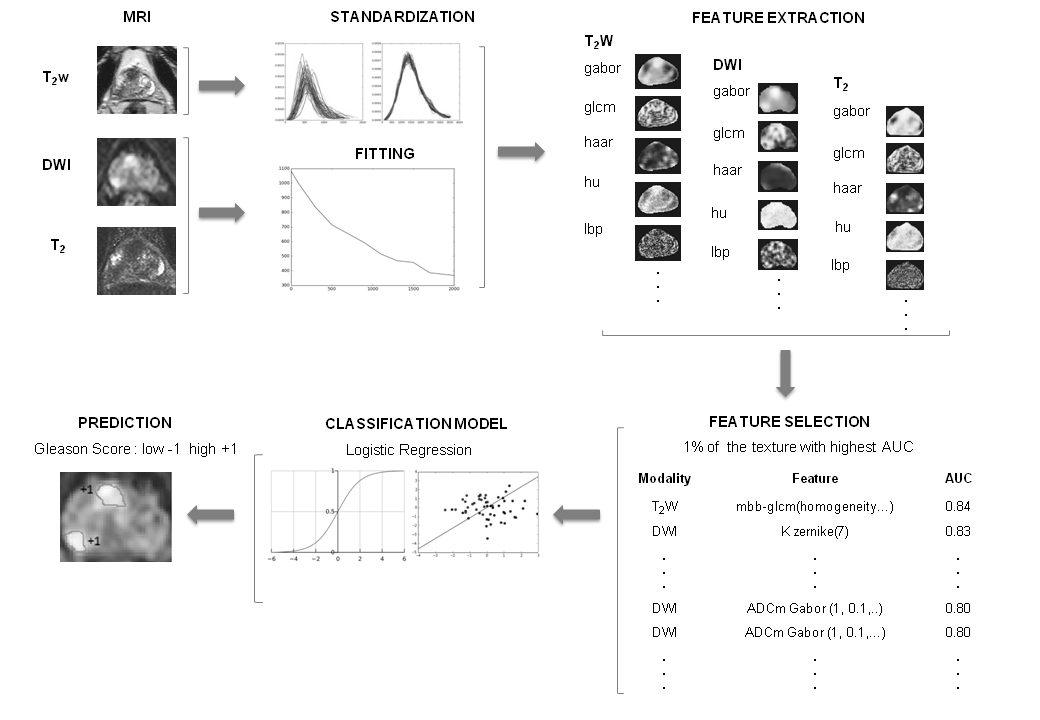
\includegraphics[width=1.0\textwidth]{figures/fig1}
    \caption{{\bf The post-processing pipeline.}
    The T₂-weighted imaging (T₂w) data set is standardized, while the
    monoexponential and kurtosis models are applied to diffusion weighted
    imaging (DWI) data set. The T₂ relaxation values are obtained using a two
    parameter monoexponential function. Subsequently, the features are
    calculated using T₂w and parametric maps. The feature selection is performed
    by choosing 1\% of the features with highest AUC\@. Then with the selected
    features a logistic regression model is fitted and used to predict the
    lesion's Gleason score group.}%
    \label{fig:pipeline}
\end{figure}

\begin{figure}[!ht]
    \centering
    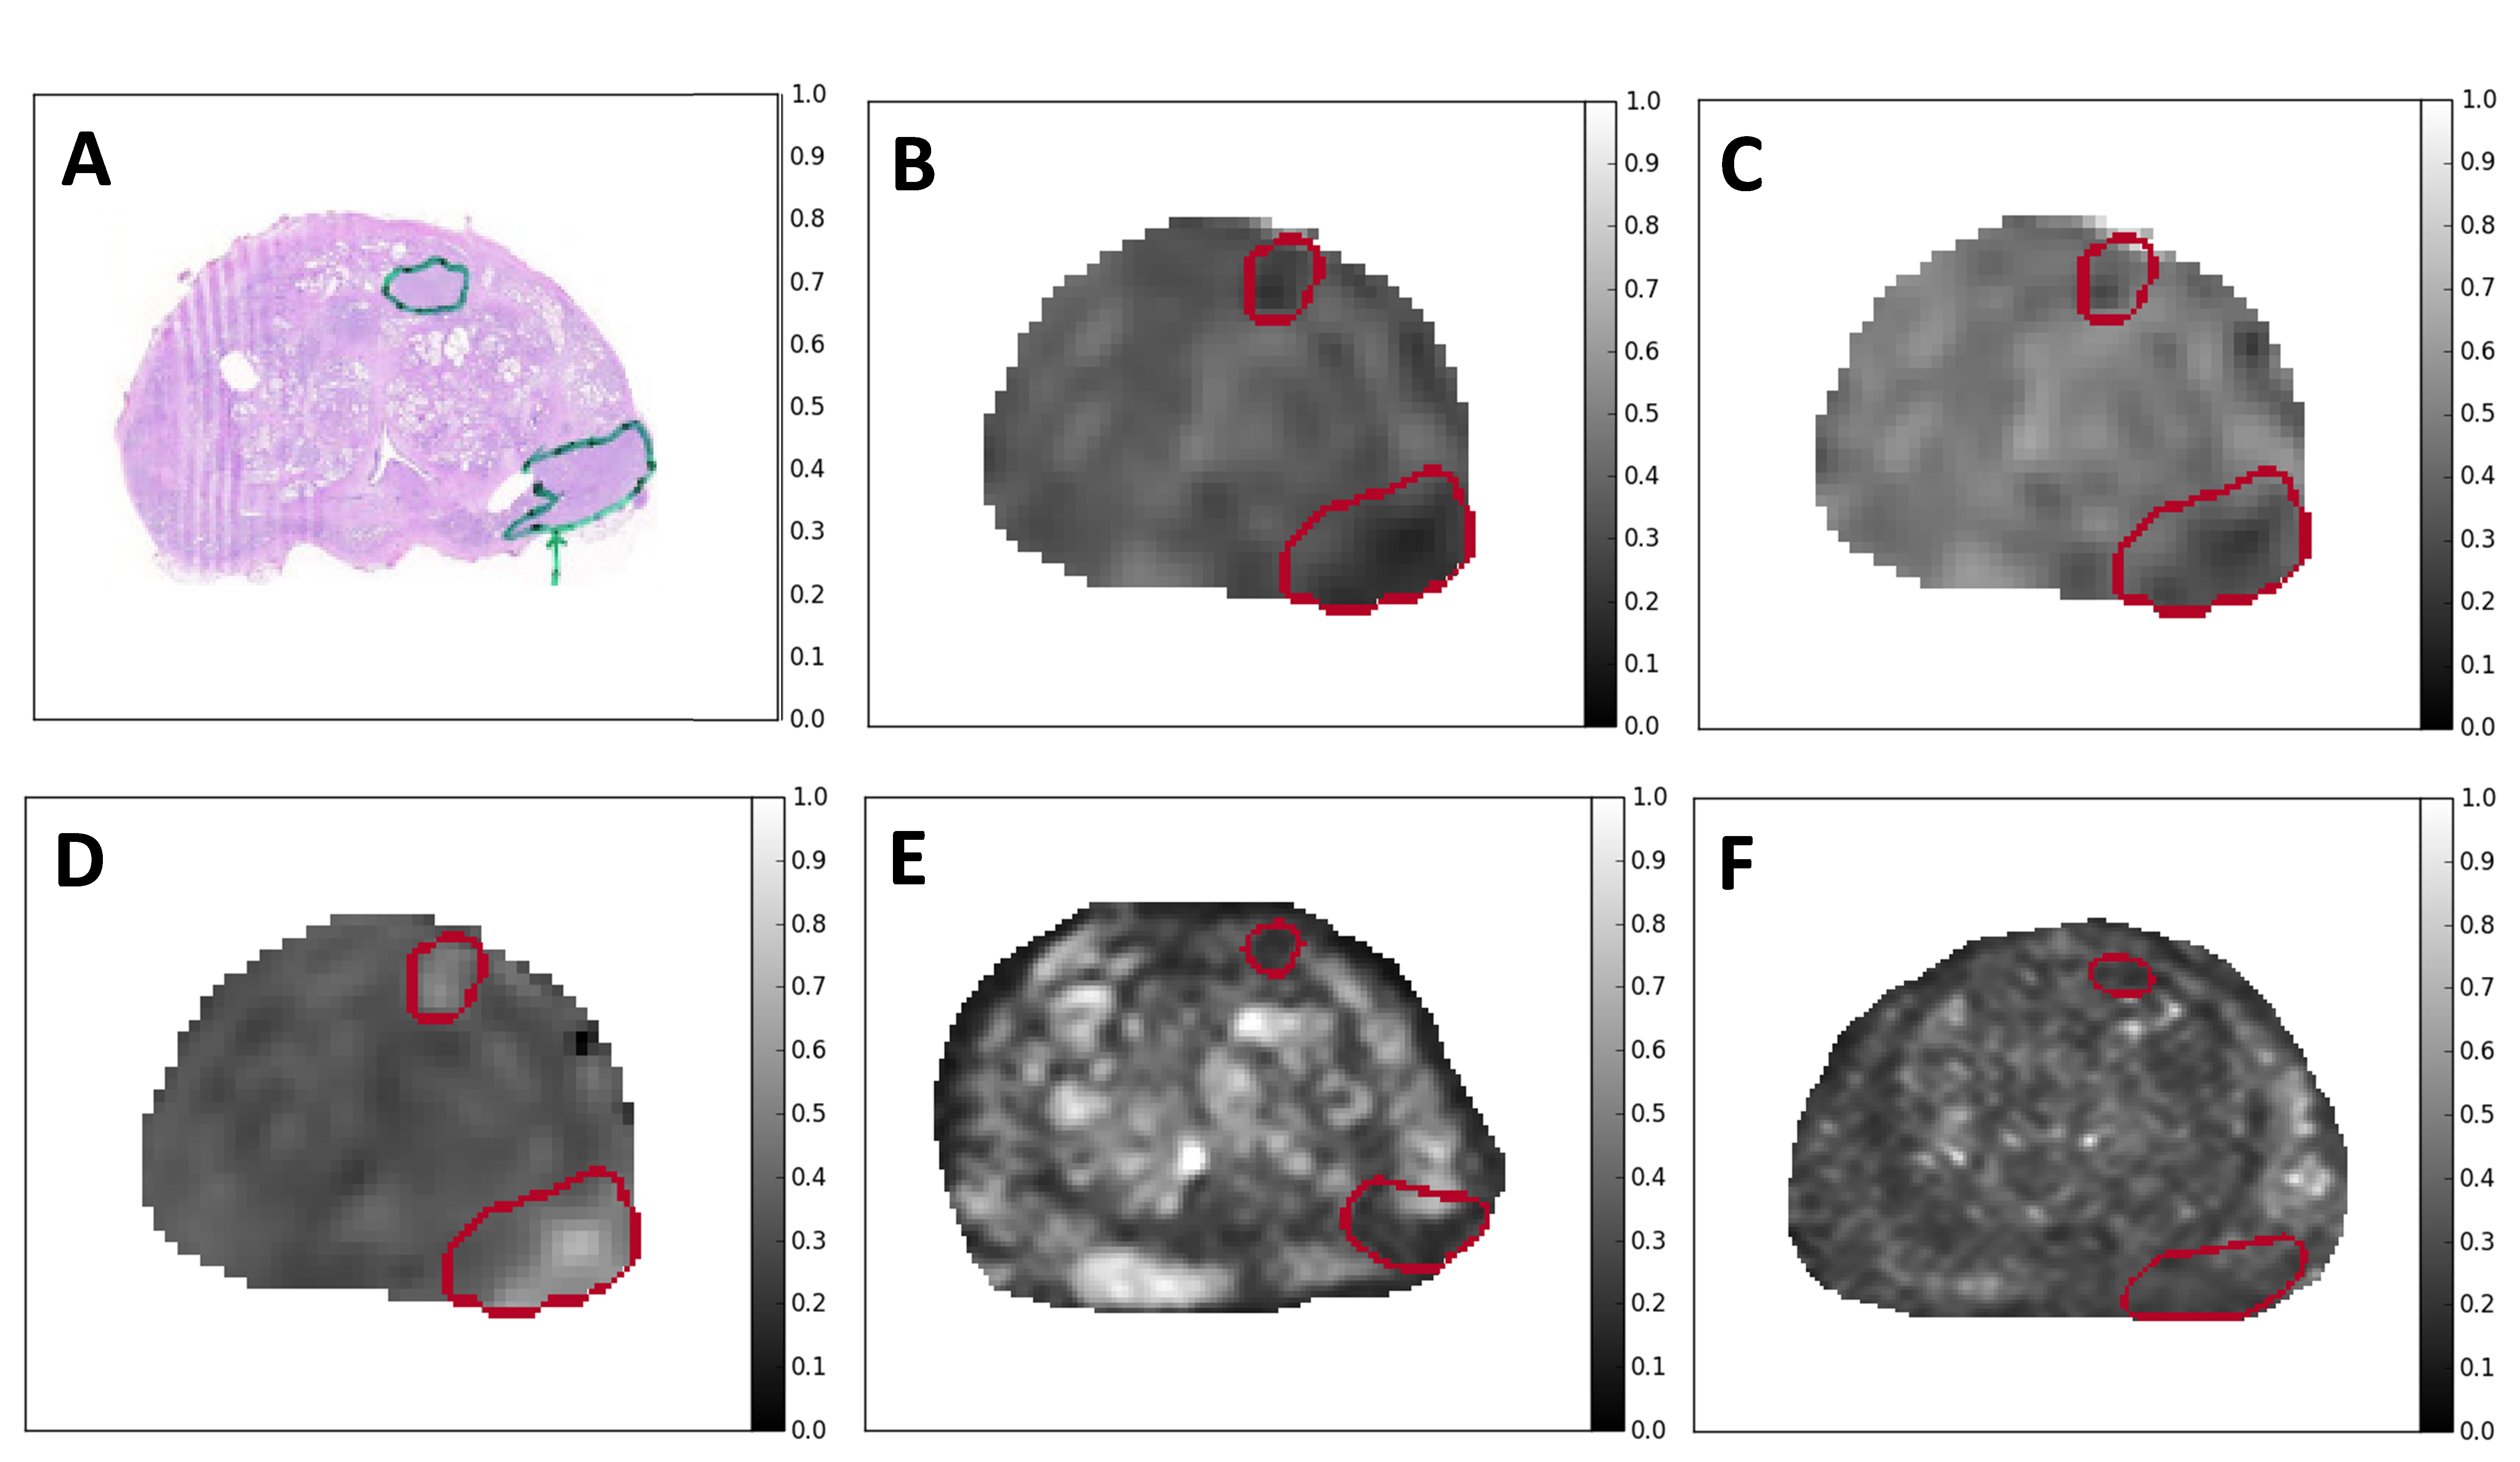
\includegraphics[width=1.0\textwidth]{figures/fig2}
    \caption{{\bf An example case with parametric maps.}
    A:~Whole mount prostate histological section.
    B:~ADCₘ. C:~ADCₖ. D:~K. E:~T₂w. F:~T₂.
    This is from patient \#43 in Table~S1. The two lesions are outlined; their
    Gleason scores are 4+3 (lower, posterolateral region) and 3+4 (upper,
    anterior region).}%
    \label{fig:pmap}
\end{figure}

\subsubsection{T₂w standardization}

The signal intensity of a T₂w image is not a specific tissue property and
this non-standardness of T₂w images (``intensity drift'') requires
standardization to a common scale. To correct this bias, a histogram alignment
method was used, as described by Nyúl et al.\ \cite{Nyul1999, Nyul2000}. This
simple method transforms the images to make their histograms match at certain
landmark locations, and interpolates the values between.

In this study, the deciles (i.e.\ every tenth percentile) were used as
landmarks, as suggested by Nyúl et al.\ \cite{Nyul1999}. Only delineated
prostate volume was considered for histogram averages, as other parts of the
image might distort the learning. The result was validated by visual inspection.

\subsubsection{DWI fitting}

Diffusion weighted imaging data sets were fitted on voxel level using the
monoexponential model:

\begin{equation}
  S(b) = S_0 \exp(-b \text{ADCₘ})
\end{equation}

and the kurtosis model \citep{Jensen2005}:

\begin{equation}
  S(b) = S_0 \exp\left(
    -b \text{ADCₖ} + \frac{1}{6} b^2 \text{ADCₖ}^2 \text{K}
  \right)
\end{equation}

where $S(b)$ is the signal intensity as a function of $b$ value, $S_0$ is the
signal intensity at $b=0$~s/mm², ADCₘ is the apparent diffusion coefficient
of the monoexponential model, ADCₖ is the apparent diffusion coefficient of
the kurtosis model, and K is the kurtosis.

The fitting procedure was performed using the Broyden-Fletcher-Goldfarb-Shanno
(BFGS) algorithm \citep{Shanno1985} implemented by the dlib \citep{King2009}
library. In order to find a reliable fit and prevent local minima, the algorithm
was executed with multiple evenly spaced initialization values. Their intervals
(step sizes) were for ADCₘ 0.1--3.0~µm²/ms (0.01~µm²/ms), for ADCₖ
0.01--3.0~µm²/ms (0.1~µm²/ms), and for K 0.0001--4.0 (0.2).

\subsubsection{T₂ fitting}

T₂ relaxation values were calculated on a single voxel level using a two
parameter monoexponential function:

\begin{equation}
  S(\TE) = S_0 \exp(-\TE / \text{T₂})
\end{equation}

where $S(\TE)$ is the signal intensity at given time $\TE$, $S_0$ is the signal
intensity at $\TE=0$~ms, and T₂ is the spin-spin relaxation time.

The Levenberg-Marquardt algorithm was used for fitting, as implemented by the
SciPy library, with the multiple initialization values of 0.0~ms to 300~ms with
step size of 50~ms. T₂ relaxation values were constrained to 1--300~ms interval.


\subsection{Feature extraction}

Texture extraction methods can be roughly categorized into four main groups
\citep{Castellano2004}, although this taxonomy is somewhat ambiguous. The
statistical approach is based on local spatial distributions and relationships
of intensity occurrences in the image. The structural methods use well-defined
geometrical primitives to measure texture. The model-based methods attempt to
represent the image properties as parameters of various mathematical models. The
transform methods use signal processing transformations such as Fourier and
wavelets to analyze the image in a different space.

In this study, the gray-level co-occurrence matrix, the local binary patterns,
and the histogram of oriented gradients can be assigned into the statistical
category, and the Sobel operator into the structural one. The Hu and Zernike
moments belong to the model-based group, while the Gabor filter and the Haar
wavelet are transform methods.

The selection of texture extraction methods used in this study was based mainly
on prior experiences in existing MRI literature \citep{Castellano2004,
Lemaitre2015} and the availability of applicable open-source software
components. All of these texture descriptor methods, except the Hu and Zernike
moments, have been previously used for CAD of PCa. However, detailed information
on their implementation and parameter selection are usually very scarce. This
issue was addressed in this study by providing complete information on the
parameters, and by using a wide array of them.

Three-dimensional texture extraction of MRI has been utilized in various
studies, including some of PCa diagnosis \citep{Depeursinge2014}. In this study,
however, texture analysis was performed only in 2D and per-slice, due to voxel
anisotropy.

\subsubsection{General implementation details}

Several texture descriptor methods with various parameter combinations were used
for extracting 2D texture features from the manually delineated PCa lesions.
Most of the methods in this study inherently incorporate the so-called ``sliding
window'' algorithm. This means that the local voxel neighborhood for
calculations is represented as a fixed-shape subwindow centered at each voxel in
turn. The output image, a texture feature map, consists of the feature values
positioned on corresponding neighborhood center locations. A more detailed
explanation is provided by Clausi et al.\ \cite{Clausi2002Rapid}, for example.

Seven window configurations were used for DWI and nine for T₂w and T₂
data. These square-shaped windows had evenly spaced voxel side lengths of 3, 5,
…, 15 for DWI and 3, 7, …, 35 for the higher-resolution T₂w and T₂. These
lengths correspond to 3.3--17 mm for DWI and 1.4--16 mm for T₂w and T₂,
maintaining similar physical cover over different resolutions.

For each lesion, the window was placed on all possible locations along the
transverse planes so that it still stayed completely within the lesion area. In
cases of the window not fitting completely inside lesion area, the window
locations with maximum lesion area were used. Extracted texture feature maps
were then averaged over all slices to be used as lesion-wise median features.
The use of different window sizes and parameter combinations resulted in 1281
features per DWI image type (ADCₘ, ADCₖ, K) and 1631 features per other image
type (T₂w, T₂), totaling 7105 features all five image types combined. The free
software libraries Scikit-image \citep{VanderWalt2014} and Mahotas
\citep{Coelho2013} were utilized in the implementation of the process.

\subsubsection{Method-specific implementation details}

The gray-level co-occurrence matrix (GLCM) \citep{Haralick1973} is a very
popular method of texture characterization. It observes all the pixel gray level
pairings that occur in the image at a certain distance and direction. In this
study, the GLCM was calculated for each window using four different voxel
distances of 1 to 4 (unless prevented by window dimensions). Because the 22
GLCM-derived features introduced by Haralick et al.\ \cite{Haralick1973} have
correlation \citep{Albregtsen2008}, using only three to five features have been
recommended \citep{Clausi2002Analysis, Albregtsen2008, Gebejes2013a} in order to
minimize redundancy and dimensionality.

In this study, the six GLCM features implemented by the Scikit-image software
library \citep{VanderWalt2014} were extracted. These features, namely contrast,
dissimilarity, homogeneity, energy, correlation, and angular second moment
(i.e.\ uniformity), are among the ones most commonly used in previous studies
\citep{Clausi2002Rapid}. They are generally considered effective texture
discriminators, and maintain invariance regarding scale and shift
\citep{Clausi2002Analysis}. In order to gain orientation invariance, the results
were averaged over four bidirectional axes, and mean range over the orientations
was added \citep{Haralick1973}.

Since GLCM requires a discrete source image, the images needed prior
normalization depending on source type. All images were quantized by uniform
scaling to 32 gray levels, based on previous studies \citep{Clausi2002Analysis,
Clausi2002Rapid, Albregtsen2008}. The image type specific source intensity
ranges for scaling were manually defined by observing prostate volume
histograms. In total 324--420 GLCM related features with sliding window approach
were extracted per image type (T₂w, ADCₘ, ADCₖ, K, T₂).

In addition to the sliding window approach, the same GLCM-based features were
also extracted using the minimum bounding box (MBB) around the whole lesion
area of each image slice as the window, while ignoring any non-lesion voxels.
This procedure is similar to the method used in a study by Vignati et
al.\ \cite{Vignati2015}. The MBB-GLCM features were averaged over slices, and
48 features in total were extracted per image type.

Local binary patterns (LBP) \citep{Ojala1996} is a method that compares every
voxel intensity value to a certain number of neighboring values on a circle
around it. Each comparison result is stored as a single bit that tells whether
the neighbor is larger or smaller than the center. The bit patterns are
collected from the neighborhood and encoded as numbers, and the resulting
histogram can then be used as a feature vector invariant to gray scale. In this
study, the LBP were calculated within each window, observing eight interpolated
neighboring points at the maximum radius allowed by window size. The different
orientations of the uniform patterns were combined into rotation-invariant
groups, and all non-uniform patterns were treated as a single pattern. Pattern
frequency histograms were then used as features resulting in 70--90 different
features per image type.

The Gabor function \citep{Gabor1946} is a Gaussian modulated by a sinusoidal
wave. Gabor filter banks can be used for texture characterization, as each
filter, shaped by its parameters, responds to specific local spatial frequency
properties of the image \citep{Turner1986}. Gabor filters are sensitive to edges
in the image, so given that different lesions contain different regions, the
detected edges between the regions could yield different responses. In this
study, the texture extraction scheme described by Tüceryan et
al.\ \cite{Tuceryan1998} was applied, which uses the sliding window on the
Gabor-filtered complex images.

Based on experimentation and data visualization, the filter bank included the
combinations of five different frequencies for the sinusoidal
($f=0.1,0.2,…,0.5$ per voxel), three sizes for a circular Gaussian
envelope ($\sigma=1,2,3$), and four bidirectional orientations. A number of
derived features have been suggested \citep{Clausi2000, Hammouda2000,
Grigorescu2002}. Here, the extracted features included mean of the real part,
variance of the real part, mean of the absolute of the real part, and mean of
the magnitude. Various ways to achieve orientation invariance have been proposed
\citep{Arivazhagan2006, Han2007, Chu2009, Rahman2011}, although not all are
equally suitable for texture classification. In this study, the simple method of
summing filtered images over orientations was used \citep{Han2007}, yielding
420--540 features per image type.

The Haar transform is a simple wavelet decomposition of the image. Providing
local spatial frequency information, it is useful as a tool of texture analysis
\citep{Lonnestad1992}. In this study, a four-level Haar transform was first done
for each image slice, and the three higher frequency coefficient planes were
used, upscaled to the original size. For each sliding window, the mean absolute
value and the standard deviation were then extracted as features
\citep{Lonnestad1992}, resulting in 168--216 features per image type.

Image moments are weighted averages that describe the distribution of intensity
within image. A few variations are widely used as object shape descriptors, but
they have also been applied to texture analysis \citep{Tuceryan1994}. In this
study, logarithms of the absolute values of the seven Hu moments \citep{Hu1962},
and the magnitude values of the complex Zernike moments \citep{Teague1980} up to
the 8th degree were calculated for each window. The Hu moments are invariant
regarding translation, scaling, rotation, and reflection
\citep{Theodoridis2003}. The Zernike moment magnitudes are rotation invariant,
robust to noise, and, due to their orthogonality, have minimal redundancy
\citep{Tahmasbi2011, Amayeh2005}. In total, 49--63 Hu moments and 175--225
Zernike moments were extracted from each image type.

The histogram of oriented gradients \citep{Dalal2005} is an algorithm developed
primarily for object recognition. It describes an object as a set of local
gradient direction distributions. In this study, it was applied for texture
analysis, using a single cell with eight directions for each window. The average
over windows was then used as a feature, resulting in one feature per window
size and 7--9 features in total per image type.

The Sobel operator \citep{Sobel1990} is a simple convolution filter that
emphasizes edges in image. The shape of the kernel window is 3×3 by definition,
so no other window sizes were used. Instead, the median of the whole lesion-wide
texture map was used, both with the lesion edge voxels included and excluded,
resulting in 2 features.

In addition, first-order statistical features were calculated over the whole
lesion. First-order statistics observe only the probabilistic distribution of
intensity values, ignoring their spatial relations. Existing literature
typically utilizes averages and some of the percentiles \citep{Shaish2016}.
Here, 18 features were included, namely mean, standard deviation, range,
minimum, maximum, quartiles, deciles, kurtosis, and skewness.


\subsection{Classification}

For image types ADCₘ, ADCₖ, and K, a corresponding data set of 100 data points and
1281 features were used to build models for predicting prostate lesion
aggressiveness based on Gleason score, while for T₂w and T₂ the number of
features was 1631. The features were normalized to zero mean and unit variance.
The data points were divided into two groups by Gleason score, low and high
(3+3 and >3+3, respectively).

Logistic regression with either L1 or L2 regularization \citep{Friedman2010}
implemented by Python Scikit-learn library \citep{Pedregosa2011} were used to
train the low vs high Gleason score classifiers. Both regularization mechanisms
compensate the high dimensionality of the data by penalizing large coefficient
values of the inferred linear models, which in turn makes them less likely to
overfit to the training data and more able to generalize to data unseen in the
training phase.

L1 regularization has the additional property of shrinking the coefficients of
the least useful features down to zero, and hence it also performs feature
selection \citep{Park2007}. The number of coefficients ending down to zero
depends on the amount of regularization. However, regularizing too strongly
might lose valuable features and lead to underfitting. Therefore, it was also
tested whether the simultaneous use of the classical filtering based feature
selection approach would improve the prediction performance.

The predictive performance of the models built by the regularized logistic
regression algorithms was estimated by a nested cross validation strategy
\citep{Varma2006}, which consisted of an outer leave-pair-out cross-validation
(LPOCV) \citep{Airola2011} and an inner 10-fold cross validation (10FCV) for
hyperparameter selection. In LPOCV every possible pair of data points were held
out at a time as test set, while the remaining data formed the training set used
to build the model for predicting on the held out pair. Both the filter based
feature selection and the hyperparameter selection were performed for each
round on LPOCV using the training set.

For selecting the best features, their performance was estimated using the
receiver operating characteristic (ROC) curve, summarized as the area under the
ROC curve (AUC). Ranked by AUC, the highest-performing 1\% of the features were
used to train the classifier.

After selecting the features the training set was transformed accordingly and
the optimum regularization hyperparameter value was selected from $\omega =
\{0.001, 0.01, 0.1, 1, 10\}$, as measured by the AUC in stratified 10FCV\@. A
classifier was then trained with the selected features and the regularization
hyperparameter, and used for performing predictions on the two data points held
out during the LPOCV round.

Afterwards, each data point was assigned an LPOCV score according to the
ordering-by-the-number-of-wins method, in which the score of a data point is the
number of times it obtains a larger predicted value than the other point during
the LPOCV rounds when it is one of the two held out points. These LPOCV scores
were then used to perform the ROC curve analysis, whose validity was previously
demonstrated by Balcan et al.\ \cite{Balcan2008}. More precisely, using the
LPOCV scores of the data points and their corresponding true label, the AUC and
95\% confidence interval (CI) were calculated using the R package by LeDell et
al.\ \cite{LeDell2015}.

The feature selection and hyperparameter selection process as part of the LPOCV
is illustrated in Pseudo code~\ref{alg:pseudocode}. The algorithm starts with a
loop referred as LPOCV\@. During this loop the indices associated with the test
pair in turn, $(i,j)$ with $i \neq j$, are not included in the index set $C$ of
training data. Every feature AUC is calculated using data from matrix $\vec{X}$
and label vector $\vec{y}$. The notation $\vec{X}[C,k]$ refers to the submatrix
of $\vec{X}$ containing the rows indexed by $C$ and the columns by $k$, that is,
the vector with the values for $k$th feature in the training data. The top 1\%
independent features are indexed by $\indx$. The optimum regularization
hyperparameter value $\alpha \in \omega$ is calculated using 10FCV on data
$(\vec{y}[C], \vec{X}[C,\indx])$, which is then used to train a model $f$ to
make predictions on the test pair $(\vec{X}[i,\indx], \vec{X}[j,\indx])$. The
last line of the pseudo code describes the calculation of LPOCV score using
ordering-by-the-number-of-wins method.

\begin{algorithm}[!h]
  \caption{{\bf LPOCV with inner feature selection by AUC filtering and
  hyperparameter selection.}}%
  \label{alg:pseudocode}

  \begin{algorithmic}
    \REQUIRE{$\vec{X}$, matrix of $n$ lesions × $F$ features}
    \REQUIRE{$\vec{y}$, vector of labels (1 high, -1 low)}
    \REQUIRE{$\omega = \{0.001, 0.01, 0.1, 1, 10\}$, set of hyperparameters}
    \ENSURE{LPOCV scores}
    \FOR[All possible lesion pairs]{$i, j \in \{1,2,\dotsc,n\}$}
      \STATE{$C \gets \{1,2,\dotsc,n\} \setminus \{i,j\}$}
          \COMMENT{All lesions except $i,j$}
      \STATE{$\vec{auc} \gets$ vector of length $F$}
      \FOR{$k \in \{1,2,\dotsc,F\}$}
        \STATE{$\vec{auc}[k] \gets \mathrm{AUC}(\vec{X}[C,k], \vec{y}[C])$}
            \COMMENT{Calculate AUC for each feature}
        \STATE{$\vec{auc}[k] \gets \max(\vec{auc}[k], 1-\vec{auc}[k])$}
            \COMMENT{Handle inverse correlation}
      \ENDFOR{}
    \STATE{$\indx \gets \arg\mathrm{sort}(\vec{auc})[1 \dotso (0.01 \times F)]$}
        \COMMENT{Get indices of the best features}
    \STATE{$\alpha \gets \mathrm{gridSearch}(\vec{y}[C], \vec{X}[C,\indx], \omega)$}
        \COMMENT{Grid search with 10FCV, returns the best hyperparameter}
    \STATE{$f \gets A(\vec{y}[C], \vec{X}[C,\indx], \alpha)$}
        \COMMENT{Train model f with algorithm A and hyperparameter $\alpha$}
    \STATE{$\vec{W}_{ij} \gets H(f(\vec{X}[i,\indx]) - f(\vec{X}[j,\indx]))$}
        \COMMENT{Matrix W stores results from Heaviside function (H) of i and j
        prediction difference}
    \ENDFOR{}
    \STATE{$\tilde{\vec{y}} \gets \vec{W} \textbf{1}$}
        \COMMENT{Score of each element obtained by summing along axis j}
    \RETURN{$\tilde{\vec{y}}$}
        \COMMENT{Returns LPOCV scores}
  \end{algorithmic}
\end{algorithm}


\subsection{Addressing bias and imbalance}

It is important to note that the nested cross-validation scheme allows feature
selection and hyperparameter tuning while avoiding bias in the performance
estimate \citep{Varma2006}. In each round of LPOCV, the pair of data points left
for testing does not affect the feature selection nor the hyperparameter tuning
of the predictive model in turn.

The ratio between low and high Gleason score is 1:4 in the data set, so there is
some degree of imbalance between classes. However, the model performance was
estimated using LPOCV together with AUC, and that degree of imbalance in the
classes has low effect on these methods \citep{Airola2011, Smith2014}. LPOCV is
an unbiased estimate of the prediction performance of a model
\citep{Airola2011}, and the ROC AUC is not affected by imbalance as it measures
how accurately a model ranks a random positive unit from a negative one
\citep{Fawcett2006}.

\section{Results}

The highest ranking features for differentiating Gleason scores are summarized
by texture extraction method in Table~\ref{tab:texture_best1p}. Features based
on Gabor filters were included in all image types. GLCM features were selected
for T₂w and T₂, and Zernike moments for K and T₂. Features from the Hu
moments and LBP were also selected for T₂, in which the top 1\% had more
variability than other image types, regarding both the texture extraction method
and window size.

\begin{table}[!h]
\begin{adjustwidth}{-2.25in}{0in}
\centering
\caption{{\bf Texture methods ranked in the best one percent.}}%
\label{tab:texture_best1p}

\begin{tabular}{c c c c}
\hline
Image type & Window sizes & Texture extraction methods & AUC range \\
\hline
T₂w & 27 & MBB-GLCM, GLCM, Gabor & 0.71--0.84 \\
ADCₘ & 11 & Gabor & 0.79--0.80 \\
ADCₖ & 11 & Gabor & 0.79--0.80 \\
K & 7, 9 & Zernike, Gabor & 0.78--0.83 \\
T₂ & 15, 19, 27, 31, 35 & Zernike, Hu, MBB-GLCM, LBP, GLCM, Gabor & 0.71--0.75 \\
\hline
\end{tabular}
\end{adjustwidth}
\end{table}


\subsection{Univariate Analysis}

ROC analysis was performed for each texture feature. The resulting best features
are shown in Table~\ref{tab:texture_imagetype}. The best one was MBB-GLCM
homogeneity in T₂w with AUC=0.84.

\begin{table}[!h]
\centering
\caption{{\bf Best texture feature per image type.}}%
\label{tab:texture_imagetype}

\begin{tabular}{c c c c}
\hline
Image type & Window sizes & Type of Texture feature & AUC \\
\hline
T₂w & NA & MBB-GLCM\@: homogeneity, $d$=3, range & 0.84 \\
ADCₘ & 11 & Gabor: $\sigma$=1, $f$=0.3, mean & 0.80 \\
ADCₖ & 11 & Gabor: $\sigma$=2, $f$=0.1, mean & 0.80 \\
K & 7 & Zernike: index=7 & 0.83 \\
T₂ & 35 & Zernike: index=3 & 0.75 \\
\hline
\end{tabular}
\end{table}

A similar analysis was performed for the first-order statistical features;
results are shown in Table~\ref{tab:stats_imagetype}. Although the best
statistical features had good performance for most of the modalities, they did
not out-perform the best texture features.

\begin{table}[!h]
\centering
\caption{{\bf Best statistical feature per image type.}}%
\label{tab:stats_imagetype}

\begin{tabular}{c c c}
\hline
Image type & Statistical feature & AUC \\
\hline
T₂w & Minimum & 0.72 \\
ADCₘ & Minimum & 0.79 \\
ADCₖ & Minimum & 0.79 \\
K & Range & 0.78 \\
T₂ & 20th percentile & 0.55 \\
\hline
\end{tabular}
\end{table}

Some of the high-ranking features are visualized in Fig~\ref{fig:tmap}. ROC
curves for best statistical and texture features are presented in
Fig~\ref{fig:roc}.

\begin{figure}[!ht]
    \centering
    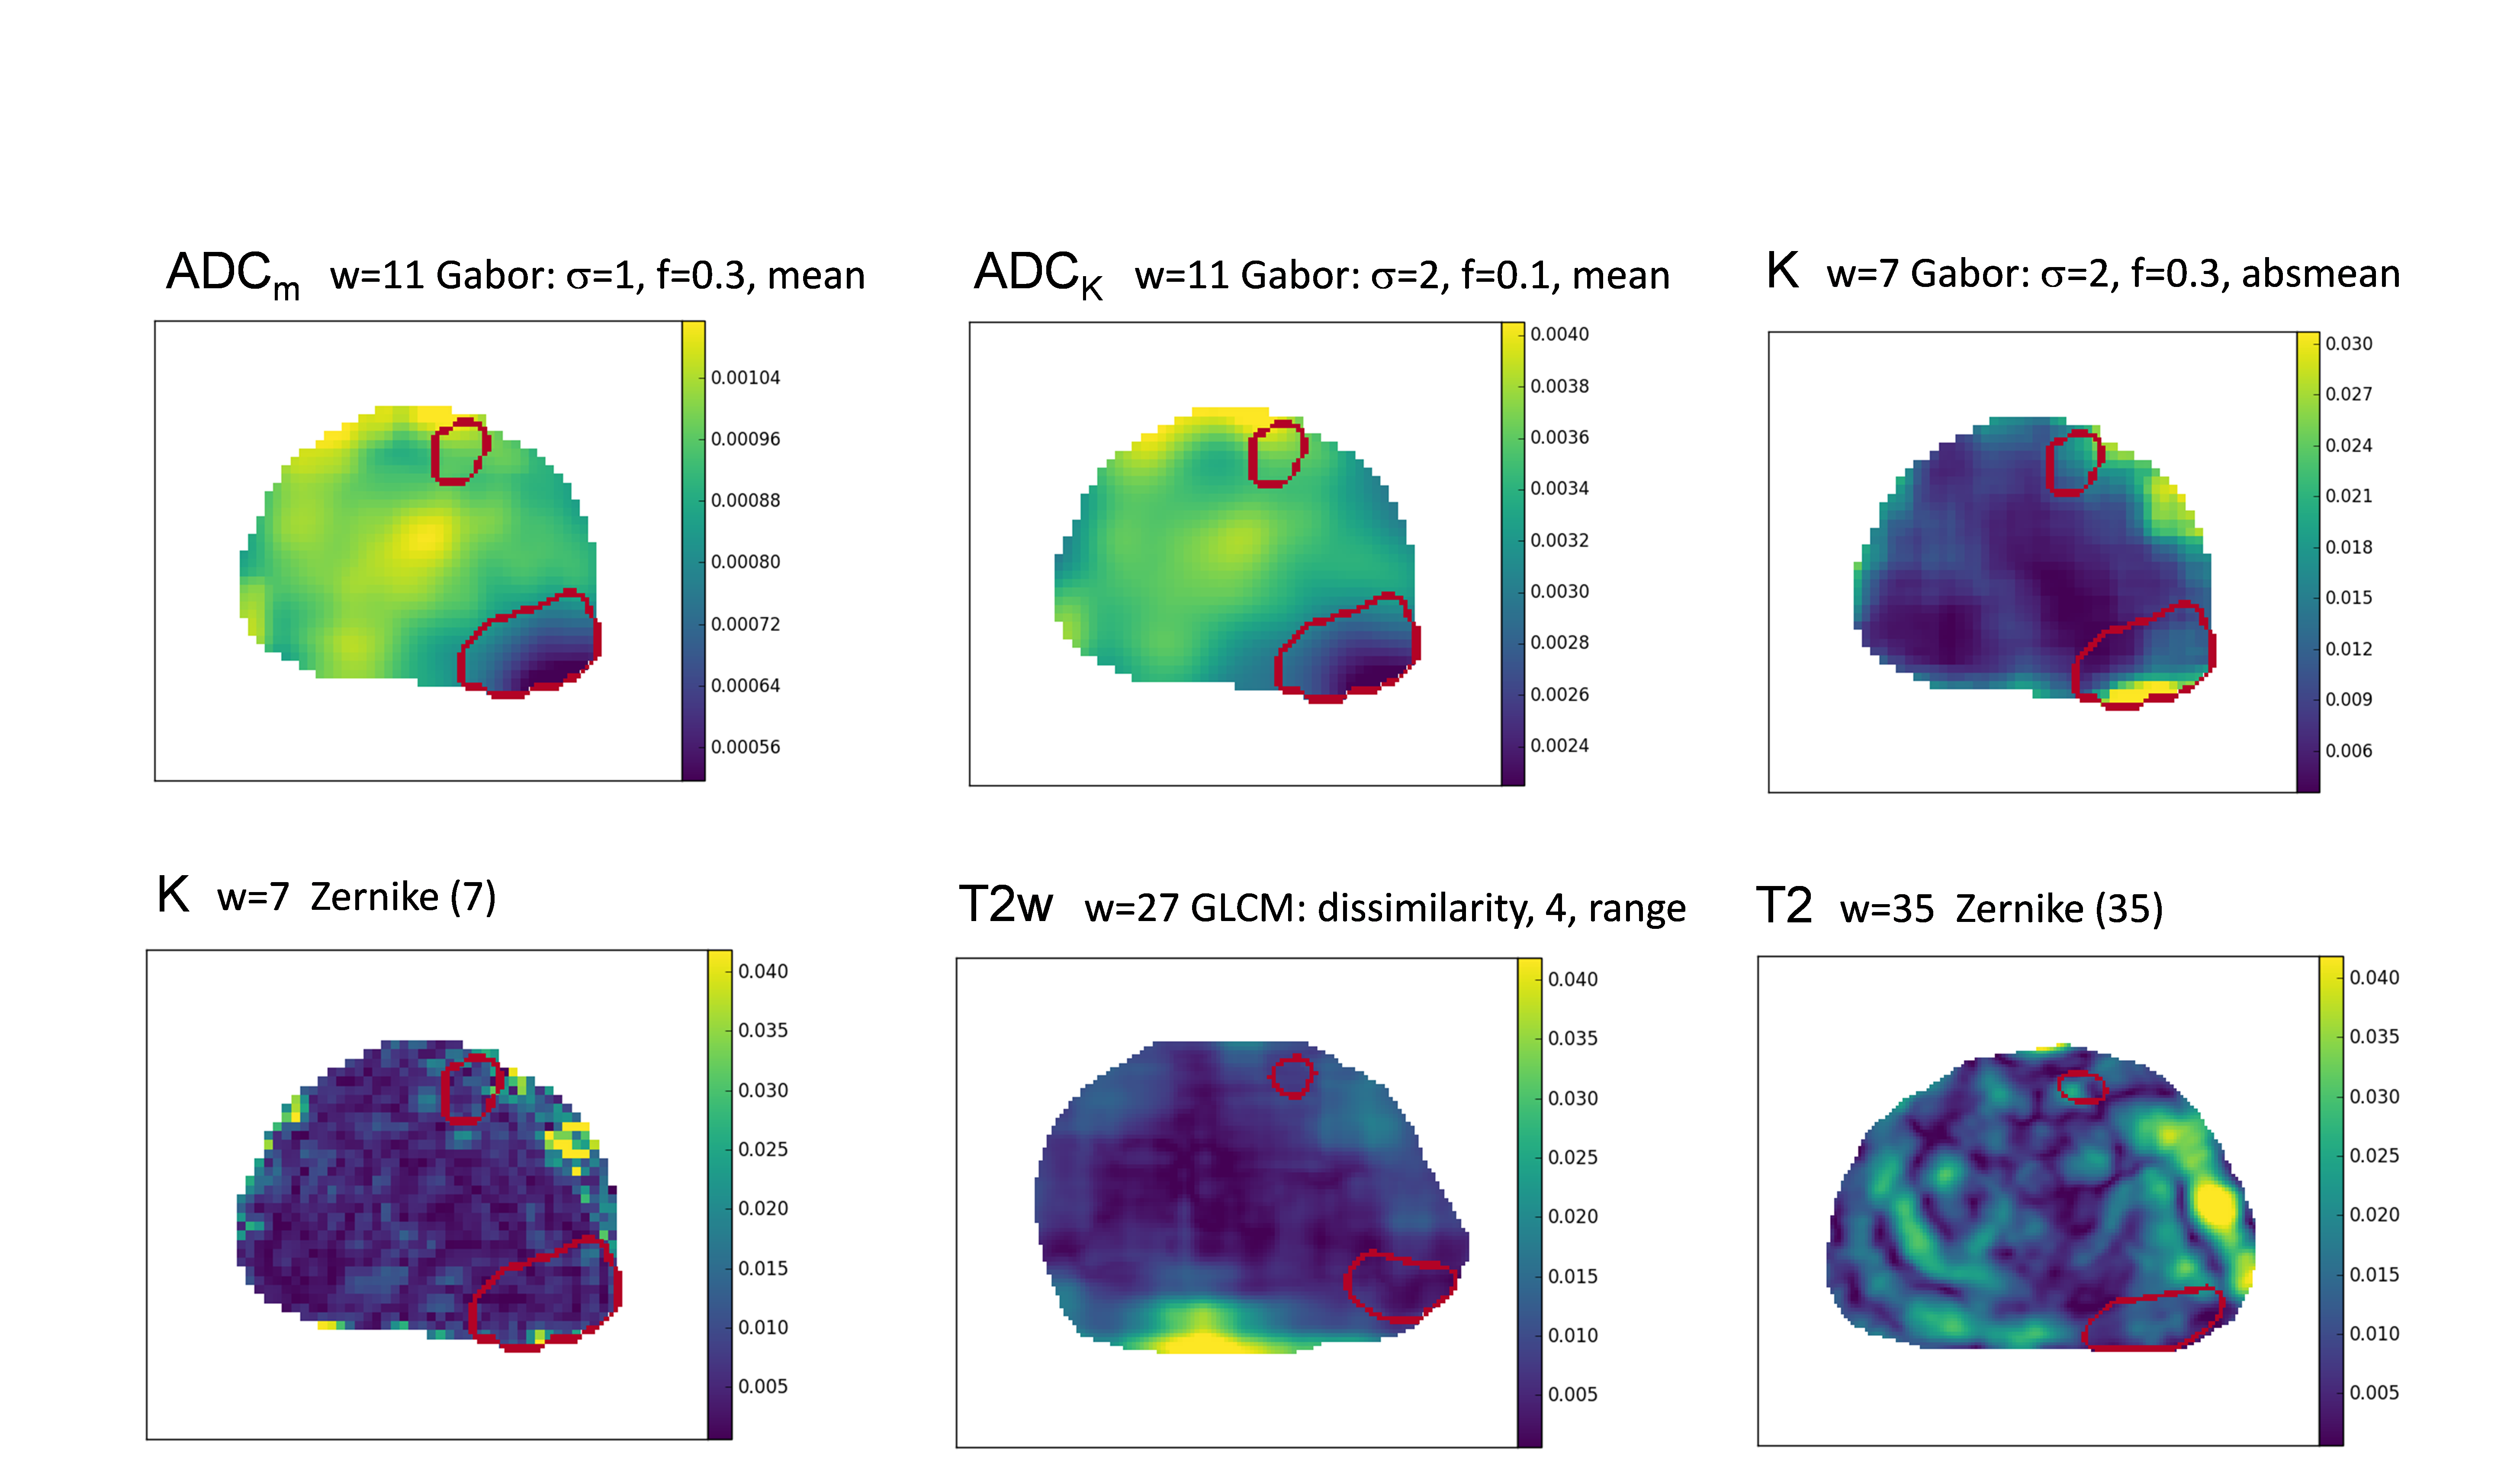
\includegraphics[width=1.0\textwidth]{figures/fig3}
    \caption{{\bf An example of texture feature maps.}
    These are extracted from DWI parametric maps (ADCₘ, ADCₖ, K), T₂-weighted
    imaging (T₂w), and parametric map of T₂ relaxation values (T₂). Source image
    type, window size, and texture descriptor parameters are shown above the
    images. The two lesions are outlined; their Gleason scores are 4+3 (lower)
    and 3+4 (upper).}%
    \label{fig:tmap}
\end{figure}

\begin{figure}[!ht]
    \centering
    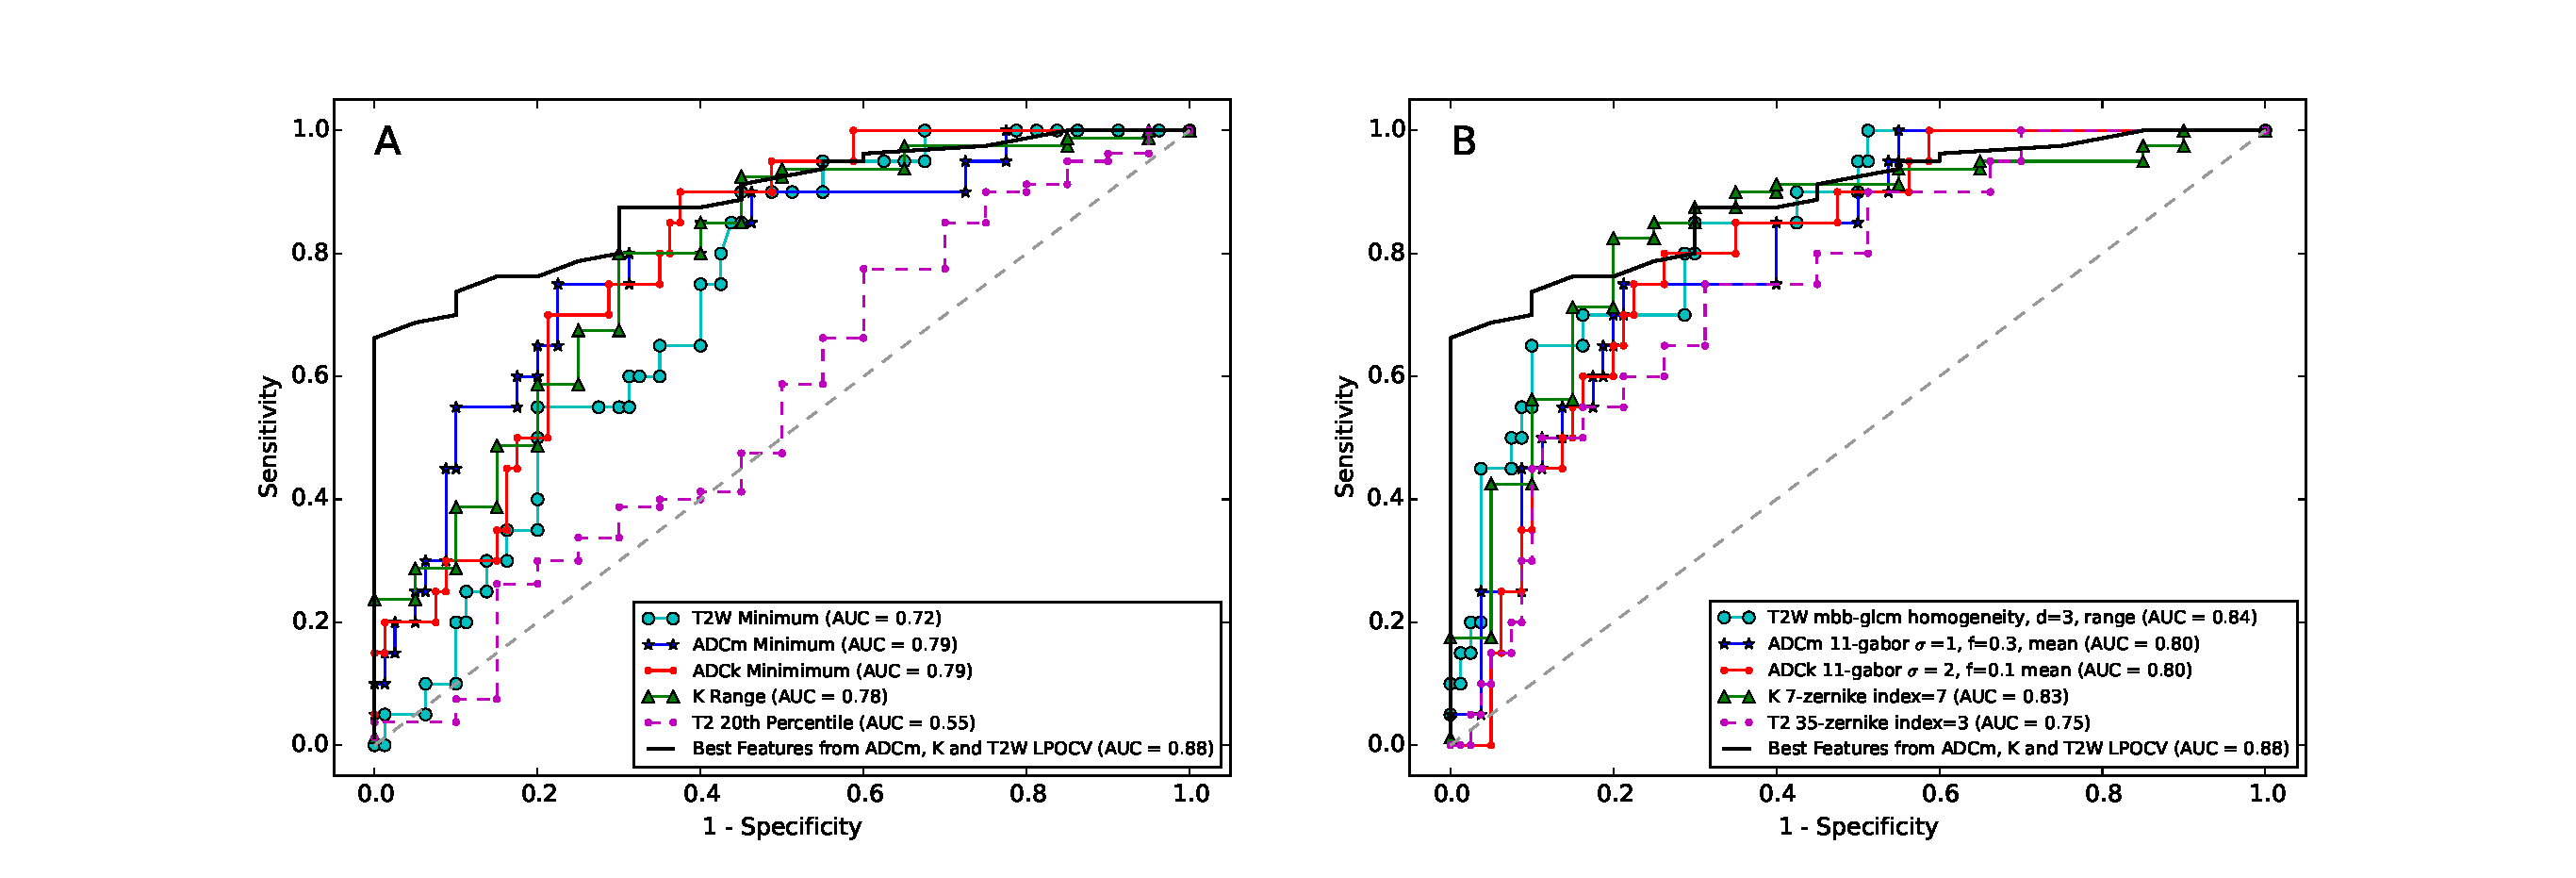
\includegraphics[width=1.0\textwidth]{figures/fig4}
    \caption{{\bf ROC curves within each image type (T₂w, ADCₘ, ADCₖ, K, T₂).}
    A:~The best statistical feature. B:~The best texture feature. The final
    model of the best selected features from ADCₘ, K, and T₂w obtained using L1
    regularized logistic regression and validated with leave-pair-out
    cross-validation (LPOCV) is also included in both A and B.}%
    \label{fig:roc}
\end{figure}


\subsection{Multivariate Analysis}

The prediction performance of the models trained using regularized logistic
regression was estimated by LPOCV\@. Both L1 and L2 regularization methods were
utilized separately. Table~\ref{tab:auc_imagetype} contains the results for
models within each image type using all of the features and top 1\% of them. The
results are presented as ROC AUC values along with 95\% confidence intervals.

\begin{table}[!h]
\begin{adjustwidth}{-2.25in}{0in}
\centering
%\caption{{\bf Area under the receiver operating curve values estimated using
%outer leave-pair-out cross-validation (LPOCV) per image type with all
%features, top 1\% features filtered by AUC, and the 18 statistical
%features.}}%
\caption{{\bf Performance figures for each image type alone.} They are ROC AUC
(receiver operating characteristic, area under curve) values estimated using
outer leave-pair-out cross-validation (LPOCV) and different feature subsets.}%
\label{tab:auc_imagetype}

%\begin{tabular}{p{3em} p{5.2em} | p{3em} p{7.2em} | p{5.7em} p{7.2em} | p{7.2em}}
\begin{tabular}{c c  c c  c c  c}
\hline
& & \multicolumn{2}{c}{All features} & \multicolumn{2}{c}{Top 1\% features} & 18 statistical \\
Image type & ML algorithm & N & AUC \ci{95\%~CI} & N & AUC \ci{95\%~CI} & AUC \ci{95\%~CI} \\
\hline
T₂w  & Log. Reg. L1 & 1631 & 0.82 \ci{0.72--0.92} & 16 & 0.80 \ci{0.69--0.90} & 0.67 \ci{0.56--0.77} \\
     & Log. Reg. L2 &      & 0.68 \ci{0.55--0.82} &    & 0.75 \ci{0.64--0.87} & 0.71 \ci{0.60--0.81} \\
ADCₘ & Log. Reg. L1 & 1281 & 0.67 \ci{0.55--0.79} & 12 & 0.71 \ci{0.60--0.82} & 0.79 \ci{0.68--0.90} \\
     & Log. Reg. L2 &      & 0.69 \ci{0.57--0.81} &    & 0.75 \ci{0.65--0.86} & 0.75 \ci{0.63--0.86} \\
ADCₖ & Log. Reg. L1 & 1281 & 0.71 \ci{0.58--0.83} & 12 & 0.74 \ci{0.63--0.84} & 0.78 \ci{0.69--0.88} \\
     & Log. Reg. L2 &      & 0.73 \ci{0.63--0.83} &    & 0.76 \ci{0.65--0.86} & 0.73 \ci{0.61--0.84} \\
K    & Log. Reg. L1 & 1281 & 0.64 \ci{0.52--0.77} & 12 & 0.78 \ci{0.67--0.89} & 0.75 \ci{0.61--0.88} \\
     & Log. Reg. L2 &      & 0.73 \ci{0.60--0.85} &    & 0.76 \ci{0.64--0.87} & 0.73 \ci{0.60--0.86} \\
T₂   & Log. Reg. L1 & 1631 & 0.58 \ci{0.45--0.71} & 16 & 0.51 \ci{0.37--0.65} & 0.67 \ci{0.55--0.79} \\
     & Log. Reg. L2 &      & 0.70 \ci{0.59--0.82} &    & 0.56 \ci{0.43--0.69} & 0.56 \ci{0.43--0.68} \\
\hline
\end{tabular}
\end{adjustwidth}
\end{table}

Similar performance estimates of the models combining features from different
image types are presented in Table~\ref{tab:auc_combinations}.

\begin{table}[!h]
\begin{adjustwidth}{-2.25in}{0in}
\centering
%\caption{{\bf Area under the receiver operating curve values estimated using
%outer leave-pair-out cross-validation (LPOCV) for the combinations of the
%image types.}}%
\caption{{\bf Performance figures for image type combinations.} They are ROC AUC
(receiver operating characteristic, area under curve) values estimated using
outer leave-pair-out cross-validation (LPOCV) and different feature subsets.}%
\label{tab:auc_combinations}

%\begin{tabular}{l p{5.2em} p{3em} p{7.2em} p{5.7em} p{7.2em}}
\begin{tabular}{c c  c c  c c}
\hline
& & \multicolumn{2}{c}{All features} & \multicolumn{2}{c}{Top 1\% features} \\
Image types & ML algorithm & N & AUC \ci{95\%~CI} & N & AUC \ci{95\%~CI} \\
\hline
ADCₖ, K                & Log. Reg. L1 & 2562 & 0.61 \ci{0.49--0.74} & 25 & 0.82 \ci{0.72--0.92} \\
                       & Log. Reg. L2 &      & 0.72 \ci{0.60--0.83} &    & 0.81 \ci{0.70--0.91} \\
ADCₘ, K                & Log. Reg. L1 & 2562 & 0.57 \ci{0.45--0.70} & 25 & 0.81 \ci{0.71--0.91} \\
                       & Log. Reg. L2 &      & 0.72 \ci{0.60--0.84} &    & 0.79 \ci{0.68--0.89} \\
ADCₘ, ADCₖ, K          & Log. Reg. L1 & 3843 & 0.58 \ci{0.44--0.72} & 38 & 0.83 \ci{0.74--0.92} \\
                       & Log. Reg. L2 &      & 0.69 \ci{0.56--0.81} &    & 0.79 \ci{0.70--0.88} \\
ADCₘ, ADCₖ, K, T₂      & Log. Reg. L1 & 5474 & 0.61 \ci{0.47--0.74} & 54 & 0.84 \ci{0.75--0.92} \\
                       & Log. Reg. L2 &      & 0.77 \ci{0.66--0.87} &    & 0.79 \ci{0.70--0.88} \\
ADCₘ, ADCₖ, K, T₂w     & Log. Reg. L1 & 5474 & 0.78 \ci{0.68--0.89} & 54 & 0.88 \ci{0.81--0.95} \\
                       & Log. Reg. L2 &      & 0.70 \ci{0.58--0.82} &    & 0.86 \ci{0.78--0.93} \\
ADCₘ, ADCₖ, K, T₂, T₂w & Log. Reg. L1 & 7105 & 0.74 \ci{0.62--0.86} & 71 & 0.88 \ci{0.81--0.95} \\
                       & Log. Reg. L2 &      & 0.79 \ci{0.69--0.90} &    & 0.86 \ci{0.78--0.93} \\
ADCₘ, K, T₂            & Log. Reg. L1 & 4193 & 0.69 \ci{0.56--0.82} & 41 & 0.83 \ci{0.74--0.91} \\
                       & Log. Reg. L2 &      & 0.78 \ci{0.68--0.88} &    & 0.82 \ci{0.73--0.90} \\
ADCₘ, K, T₂w           & Log. Reg. L1 & 4193 & 0.81 \ci{0.71--0.91} & 41 & 0.88 \ci{0.82--0.95} \\
                       & Log. Reg. L2 &      & 0.70 \ci{0.59--0.82} &    & 0.86 \ci{0.79--0.93} \\
ADCₘ, K, T₂, T₂w       & Log. Reg. L1 & 5824 & 0.76 \ci{0.65--0.87} & 58 & 0.87 \ci{0.81--0.94} \\
                       & Log. Reg. L2 &      & 0.79 \ci{0.68--0.89} &    & 0.85 \ci{0.77--0.92} \\
ADCₖ, K, T₂            & Log. Reg. L1 & 4193 & 0.53 \ci{0.40--0.66} & 41 & 0.81 \ci{0.72--0.91} \\
                       & Log. Reg. L2 &      & 0.80 \ci{0.71--0.89} &    & 0.81 \ci{0.71--0.91} \\
ADCₖ, K, T₂w           & Log. Reg. L1 & 4193 & 0.81 \ci{0.72--0.91} & 41 & 0.85 \ci{0.77--0.93} \\
                       & Log. Reg. L2 &      & 0.72 \ci{0.61--0.84} &    & 0.84 \ci{0.76--0.92} \\
T₂, T₂w                & Log. Reg. L1 & 3262 & 0.82 \ci{0.73--0.91} & 32 & 0.66 \ci{0.52--0.79} \\
                       & Log. Reg. L2 &      & 0.78 \ci{0.68--0.88} &    & 0.61 \ci{0.48--0.74} \\
\hline
\end{tabular}
\end{adjustwidth}
\end{table}


\subsubsection{All features within individual image types}

When using all features and L1 regularization (Table~\ref{tab:auc_imagetype}),
T₂w had AUC=0.82, DWI derived parametric maps (ADCₘ, ADCₖ, K) had AUC range
0.64--0.71, and T₂ derived features had AUC=0.58.

In contrast to L1, L2 regularization yielded better performance for all image
types except T₂w where AUC dropped to 0.68. DWI-derived parametric maps (ADCₘ,
ADCₖ, K) had AUC range 0.69--0.73, and T₂ derived features had AUC=0.70.

These results indicate that, when it comes to logistic regression models, all
features weighted by L2 regularization may perform better than fewer features
selected by L1, with the exception of T₂w images. With T₂w, L1 regularization
performed better than L2, suggesting that a subset of features would perform
better than all of them.


\subsubsection{Selected features within individual image types}

The feature selection was based on filtering features by AUC\@. Only the best
1\% of features (12 or 16 features, depending on image modality) with highest
ranking AUC were selected in each image type. When using L1 regularization, the
best T₂w features showed better performance (AUC=0.80) than the features of
DWI-derived parametric maps (ADCₘ, ADCₖ, K), which had AUC range 0.71--0.78. The
best T₂ features had AUC=0.51 which is the lowest performance among the
modalities.

The estimated AUC values using L2 regularization and the best 1\% features,
compared with L1 regularization, were lower for T₂w and K.

The texture features did not substantially out-perform the 18 statistical
features the corresponding image type (Table~\ref{tab:auc_imagetype}), except in
T₂w where the texture feature model obtained with L1 regularization had the best
performance among all other models. The highest AUC value based on statistical
features was 0.79, achieved using L1 regularization and ADCₘ. The corresponding
value for the best 1\% texture features was 0.71.

The AUC values for the top-1\% texture features based on T₂w, ADCₘ, ADCₖ, K,
and T₂ are shown in supporting material Tables S2, S4, S6, S8, and S10,
respectively. Similarly, AUCs for the statistical features for each image
type are shown in supporting material Tables S3, S5, S7, S9, and S11.


\subsubsection{All features of combined image types}

No substantial improvements of AUC values were present when combining all
features of all image types (Table~\ref{tab:auc_combinations}). The AUCs were
within range 0.53--0.82 with L1 regularization and within 0.69--0.80 with L2.


\subsubsection{Selected features of combined image types}

In contrast to the use all features, a better model performance was present when
combining the best 1\% features of all image types (T₂w, ADCₘ, ADCₖ, K,
T₂). The best performing model with AUC=0.88 was obtained when selecting the
best 1\% features based on ADCₘ, K and T₂w. The combinations of features
extracted from DWI parametric maps (ADCₘ, ADCₖ, K) and those extracted from T₂w
and T₂ together with the feature selection method lead to improved prediction
performance regardless of the regularization method (L1, L2).

The final model proposed to differentiate low from high Gleason score PCa
includes the features from ADCₘ, K, and T₂w listed in Table~S12. The expected
performance ROC is presented in Fig~\ref{fig:roc}.

\section{Discussion}

There is an increasing number of research groups studying and developing CAD of
prostate cancer. The topic was recently reviewed by \citet{Lemaitre2015}. Most
of the publications have focused on the task of cancer detection rather than
characterization. However, both are required for proper treatment decision
planning. In this study, we built a classifier for prostate cancer
characterization utilizing texture features extracted from T₂w, the
monoexponential and kurtosis models of high-b-value DWI, and T₂ maps.

Several studies have demonstrated correlation between ADCₘ values and Gleason
score based on biopsy \citep{Turkbey2011, Tamada2008} or prostatectomy specimens
\citep{Toivonen2015, Peng2013, Boesen2015, Rosenkrantz2015, Donati2014}. Most of
the studies evaluating the performance of DWI for Gleason score prediction have
used first-order statistical features, which do not consider the spatial
relationships between voxels. Analyzing the texture may add useful information
regarding tumor heterogeneity and other structural properties. In our previous
studies we observed rectangular, fixed-shape regions-of-interest, and each tumor
was characterized by only one variable per image type \citep{Toivonen2015,
Jambor2015Relaxation, Jambor2015Rotating}. However, in this study we measured
the texture properties of each of the image types (T₂w, ADCₘ, ADCₖ, K, T₂).
We have shown that the characterization performance of prostate cancer can be
improved by combining texture features from the monoexponential and kurtosis
models, and the T₂w.

Most studies on texture analysis of PCa include only a small number of texture
descriptors and configurations \citep{Kwak2015, Viswanath2012, Ginsburg2014}. In
this study, we utilized a large number of both, from multiparametric source.
This allows evaluating a huge number of feature combinations.

Texture analysis of multiparametric MRI has previously seen limited use in PCa
characterization. \citet{Fehr2015} evaluated PCa characterization with the
whole-lesion 1st order statistics and GLCM texture features from a similar-size
dataset of ADC and T₂w. They used oversampling to ward off effect of class
imbalance. Similarly to our study, they integrated dynamic feature selection as
part of the training (using the recursive feature selection support vector
machine, RFE-SVM). In our study, we included a much more diverse and numerous
set of features, as one of our goals was to evaluate various texture extraction
methods. Moreover, we have for the first time demonstrated that using texture
features from K (kurtosis function) provided improvements to ADCₘ
(monoexponential function). This is important since first order statistics of
parameters derived from kurtosis function do not lead to improved performance of
ADCm (monoexponential function). The effect of noise remains to be explored in
future studies.

\citet{Tiwari2013} classified PCa using GLCM and simple gradient features from
T₂w and MR spectroscopy (MRS). A multi-kernel classifier with graph embedding
was used to reduce dimensionality. \citet{Tiwari2013} had fewer patients
compared to the current study. Moreover, the classification was done on
equally-sized, rectangular metavoxels.

Furthermore, \citet{Wibmer2015} studied the associations of Gleason scores and
individual GLCM features from ADC and T₂w of PZ lesions, using generalized
linear regression and generalized estimating equations; and \citet{Vignati2015}
tested Gleason score differentiation using two of the GLCM features (contrast
and homogeneity) from T₂w and ADC individually.

Contrarily to previous approaches to performing non-rigid deformation and
co-registration of datasets with subsequent resampling to common space and
resolution \citep{Viswanath2012, Ginsburg2014}, in the current study the
prostate and tumor masks were done for each MR imaging method (T₂w, DWI, T₂)
individually, allowing us to perform texture analyses at their original native
resolutions. Estimating the effect of co-registration and resampling on texture
extraction is not trivial, and the process could cause loss of information.
However, the accuracy of the delineations in this study could be potentially
improved by an added step of co-registering MRI to histology images
\citep{Bourne2017}. We highlight the limitation of performing re-slicing and
non-rigid deformation of MR data sets to common space and then co-registering
with whole mount prostatectomy sections. As correctly noted by
\citet{Bourne2017}, co-registration of whole mount prostatectomy sections to MRI
data sets is important. However, the effect of re-slicing and non-rigid
deformation of MR data sets to common space remains to be explored.

The gray-level co-occurrence matrix may well be the most widely used tool for
texture analysis of prostate MRI data sets. The Sobel operator, Gabor filters,
Haar transform, and local binary patterns have already extensively been applied
for texture analysis of prostate MRI, as have a few others~\citep{Lemaitre2015}
not included in this study.

The image moments, on the other hand, have been used more often for global
morphological analysis like shape recognition rather than local texture
analysis, although they have been used for texture as well~\citep{Tuceryan1994,
Laws1980, Tuceryan1990}. To the best of our knowledge, there are no published
studies using moment-based texture analysis for detection or characterization of
prostate cancer using MRI data sets. \citet{Tahmasbi2011} used Zernike moments
to characterize breast cancer, but as a global mass descriptor and not for
texture. Our results suggest that moment-based texture features might be
valuable for PCa characterization. More specifically, the best 1\% features of
the image types K and T₂, and the final model ADCₘ, K, and T₂w combined
included some of the texture features based on Hu or Zernike moments.

The GLCM summarizes pixel intensity occurrences, the Gabor descriptors detect
gradients of certain frequencies, and the LBP responds to point-like intensity
transformation patterns. The image moments describe the mass distribution of the
image content which is seen as a function that is integrated over space. Given
the supposed difference in tissue heterogeneity, it makes sense that a metric
based on mass distribution would discriminate lesions of varying Gleason scores.

Most of the texture extraction methods in this study use the sliding window
algorithm with seven or nine different window sizes depending on image
resolution. Usually, the window should be large enough to provide reliable
statistical information about its contents to characterize the texture, yet
small enough so that patches of different classes do not overlap too much
\citep{Haralick1973, Clausi2002Analysis}. The nature of each texture extraction
algorithm also affects the specific role and usefulness of each window
configuration. The optimal window size depends on method and data, and typically
cannot be estimated in practice without experimentation \citep{Puig2001}. Most
of the previous studies have utilized a very small number of different window
sizes, often without presenting validation for the choice. In this study, we
explored several window sizes simultaneously. This approach greatly increases
the number of features, which is usually something to be avoided in order to
produce an effective classifier. However, the machine learning method we used
scales well to a large number of features.

We have evaluated an extensive number of MRI texture features in multivariate
setting for their ability to predict the Gleason score of prostate cancer.
Moreover, we have presented a machine learning system that, from a very large
number of candidate features, searches for a relevant subset for the task and
alternatively weights the features accordingly. The single feature with highest
prediction performance estimate (AUC = 0.84) was a gray-level co-occurrence
matrix homogeneity of T₂w. The Gabor transform features performed well with the
ADC and K parameters. The lowest percentile statistics were useful with ADC and
T₂w. The features based on Hu and Zernike moments performed well for K and T₂.
Our results imply that a specific set of features and feature extraction methods
is needed to obtain maximal information from DWI, T₂w, and T₂. The highest
overall performance estimate (AUC = 0.88) was obtained for the model utilizing a
small subset of texture features from the ADCₘ, K, and T₂w parameters. These
features included texture descriptors based on gray-level co-occurrence matrix,
Gabor transform, and the Zernike and Hu moments.

Our study has several limitations. First of all, only 62 patients were included
and further validation of our results in large patient cohort is needed. All of
the patients had gone through prostatectomy, and therefore it is biased on the
high Gleason score group with 80\% of the lesions. As is the case with many
previous studies, only one MRI data set per imaging method per patient was
evaluated. Therefore, the repeatability of the texture features cannot be
evaluated. Ideally, quantitative imaging methods would have high reliability and
repeatability, allowing the use of derived features for disease characterization
\citep{Shrout1979}.

Many of the texture extraction methods used in this study could be further
refined. Variations of the methods and the derived features have been proposed,
for example for Gabor filters \citep{Clausi2000}, and local binary patterns
\citep{Guo2012, Maenpaa2003}. For Gabor filters, schemes for unsupervised tuning
of optimal parameters have been proposed \citep{Teuner1995}. The Zernike moments
can be provided scale and transformation invariance \citep{Khotanzad1990}.

In the cross-validation process the set of selected features was slightly
different in every round, implying that some of the features may convey similar
information. This is natural since we tested such a large number of feature
candidates.

In this study, we focused on the characterization of histologically confirmed
and manually delineated cancer lesions. In a more practical setting, this
process should be preceded by automatic segmentation of the prostate and
detection of cancerous tissue. This limitation should be addressed in future
studies.

Studies show increased risk of PCa specific mortality for Gleason score 4+3 in
comparison to 3+4~\citep{Wright2009}. Differentiating these scores in the
characterization process would be useful in addition to the 3+3 vs >3+3
threshold that was considered in this study.

Our results suggest that the use of texture features extracted from T₂w, ADCₘ,
and K parametric maps leads to improved PCa characterization accuracy compared
to the more commonly used statistical features of DWI. In contrast, adding
features from T₂ did not improve the classification accuracy. The results
point out certain features and feature combinations that were succesful, out of
a very numerous set that includes various source image types, texture extraction
methods, window sizes, and method-specific configurations. Most of the useful
methods have already performed well in other studies (GLCM, Gabor, LBP).
However, the image moment based texture features (Hu, Zernike) appear to be
novel in the context of PCa characterization.

\section{Acknowledgements}

This study was financially supported by grants from Instrumentarium Research
Foundation, Sigrid Jusélius Foundation, Turku University Hospital, TYKS-SAPA
research fund, Finnish Cancer Society, Finnish Cultural Foundation, and Orion
Research Foundation. PT was supported by a Clinical Researcher Funding from the
Academy of Finland. We thank Jaakko Liippo (Turku University Hospital, Turku,
Finland) for his help in scanning the histological slides, and Anitta Entonen
(Turku University Hospital, Turku, Finland) for her help with patient enrollment
and assistance during MRI examinations.

\section{Tables}

\newcommand{\ci}[1]{{\small (#1)}}  % CI range for the AUCs.

\begin{algorithm}[ht]
  \caption{LPOCV with inner feature selection by AUC filtering and
  hyperparameter selection.}
  \label{alg:pseudocode}

  \begin{algorithmic}
    \REQUIRE $\vec{X}$, matrix of $n$ lesions × $F$ features
    \REQUIRE $\vec{y}$, vector of labels (1 high, -1 low)
    \REQUIRE $\omega = \{0.001, 0.01, 0.1, 1, 10\}$, set of hyperparameters
    \ENSURE LPOCV scores
    \FOR[All possible lesion pairs]{$i, j \in \{1,2,\dotsc,n\}$}
      \STATE $C \gets \{1,2,\dotsc,n\} \setminus \{i,j\}$  \COMMENT{All lesions except $i,j$}
      \STATE $\vec{auc} \gets$ vector of length $F$
      \FOR{$k \in \{1,2,\dotsc,F\}$}
        \STATE $\vec{auc}[k] \gets \mathrm{AUC}(\vec{X}[C,k], \vec{y}[C])$  \COMMENT{Calculate AUC for each feature}
        \STATE $\vec{auc}[k] \gets \max(\vec{auc}[k], 1-\vec{auc}[k])$  \COMMENT{Handle inverse correlation}
      \ENDFOR
    \STATE $\indx \gets \arg\mathrm{sort}(\vec{auc})[1 \dotso (0.01 \times F)]$  \COMMENT{Get indices of the best features}
    \STATE $\alpha \gets \mathrm{gridSearch}(\vec{y}[C], \vec{X}[C,\indx], \omega)$  \COMMENT{Grid search with 10FCV, returns the best hyperparameter}
    \STATE $f \gets A(\vec{y}[C], \vec{X}[C,\indx], \alpha)$  \COMMENT{Train model f with algorithm A and hyperparameter $\alpha$}
    \STATE $\vec{W}_{ij} \gets H(f(\vec{X}[i,\indx]) - f(\vec{X}[j,\indx]))$  \COMMENT{Matrix W stores results from Heaviside function (H) of i and j prediction difference}
    \ENDFOR
    \STATE $\tilde{\vec{y}} \gets \vec{W} \textbf{1}$  \COMMENT{Score of each element obtained by summing along axis j}
    \RETURN $\tilde{\vec{y}}$  \COMMENT{Returns LPOCV scores}
  \end{algorithmic}
\end{algorithm}


\begin{table}[ht]
  \caption{Texture methods ranked in the best one percent.}
  \label{tab:texture_best1p}

  \begin{tabular}{c c c c}
  \hline
  Image type & Window sizes & Texture extraction methods & AUC range \\
  \hline
  T₂w & 27 & MBB-GLCM, GLCM, Gabor & 0.71--0.84 \\
  ADCₘ & 11 & Gabor & 0.79--0.80 \\
  ADCₖ & 11 & Gabor & 0.79--0.80 \\
  K & 7, 9 & Zernike, Gabor & 0.78--0.83 \\
  T₂ & 15, 19, 27, 31, 35 & Zernike, Hu, MBB-GLCM, LBP, GLCM, Gabor & 0.71--0.75 \\
  \hline
  \end{tabular}
\end{table}


\begin{table}[ht]
  \caption{Best texture feature per image type.}
  \label{tab:texture_imagetype}

  \begin{tabular}{c c c c}
  \hline
  Image type & Window sizes & Type of Texture feature & AUC \\
  \hline
  T₂w & NA & MBB-GLCM\@: homogeneity, $d$=3, range & 0.84 \\
  ADCₘ & 11 & Gabor: $\sigma$=1, $f$=0.3, mean & 0.80 \\
  ADCₖ & 11 & Gabor: $\sigma$=2, $f$=0.1, mean & 0.80 \\
  K & 7 & Zernike: index=7 & 0.83 \\
  T₂ & 35 & Zernike: index=3 & 0.75 \\
  \hline
  \end{tabular}
\end{table}


\begin{table}[ht]
  \caption{Best statistical feature per image type.}
  \label{tab:stats_imagetype}

  \begin{tabular}{c c c}
  \hline
  Image type & Statistical feature & AUC \\
  \hline
  T₂w & Minimum & 0.72 \\
  ADCₘ & Minimum & 0.79 \\
  ADCₖ & Minimum & 0.79 \\
  K & Range & 0.78 \\
  T₂ & 20th percentile & 0.55 \\
  \hline
  \end{tabular}
\end{table}

\begin{table}[ht]
  \caption{Area under the receiver operating curve values estimated using outer
  leave-pair-out cross-validation (LPOCV) per image type with all features, top
  1\% features filtered by AUC, and the 18 statistical features.}
  \label{tab:auc_imagetype}

  %\begin{tabular}{p{3em} p{5.2em} | p{3em} p{7.2em} | p{5.7em} p{7.2em} | p{7.2em}}
  \begin{tabular}{c c  c c  c c  c}
  \hline
  & & \multicolumn{2}{c}{All features} & \multicolumn{2}{c}{Top 1\% features} & 18 statistical \\
  Image type & ML algorithm & N & AUC \ci{95\%~CI} & N & AUC \ci{95\%~CI} & AUC \ci{95\%~CI} \\
  \hline
  T₂w  & Log. Reg. L1 & 1631 & 0.82 \ci{0.72--0.92} & 16 & 0.80 \ci{0.69--0.90} & 0.67 \ci{0.56--0.77} \\
       & Log. Reg. L2 &      & 0.68 \ci{0.55--0.82} &    & 0.75 \ci{0.64--0.87} & 0.71 \ci{0.60--0.81} \\
  ADCₘ & Log. Reg. L1 & 1281 & 0.67 \ci{0.55--0.79} & 12 & 0.71 \ci{0.60--0.82} & 0.79 \ci{0.68--0.90} \\
       & Log. Reg. L2 &      & 0.69 \ci{0.57--0.81} &    & 0.75 \ci{0.65--0.86} & 0.75 \ci{0.63--0.86} \\
  ADCₖ & Log. Reg. L1 & 1281 & 0.71 \ci{0.58--0.83} & 12 & 0.74 \ci{0.63--0.84} & 0.78 \ci{0.69--0.88} \\
       & Log. Reg. L2 &      & 0.73 \ci{0.63--0.83} &    & 0.76 \ci{0.65--0.86} & 0.73 \ci{0.61--0.84} \\
  K    & Log. Reg. L1 & 1281 & 0.64 \ci{0.52--0.77} & 12 & 0.78 \ci{0.67--0.89} & 0.75 \ci{0.61--0.88} \\
       & Log. Reg. L2 &      & 0.73 \ci{0.60--0.85} &    & 0.76 \ci{0.64--0.87} & 0.73 \ci{0.60--0.86} \\
  T₂   & Log. Reg. L1 & 1631 & 0.58 \ci{0.45--0.71} & 16 & 0.51 \ci{0.37--0.65} & 0.67 \ci{0.55--0.79} \\
       & Log. Reg. L2 &      & 0.70 \ci{0.59--0.82} &    & 0.56 \ci{0.43--0.69} & 0.56 \ci{0.43--0.68} \\
  \hline
  \end{tabular}
\end{table}


\begin{table}[ht]
  \caption{Area under the receiver operating curve values estimated using outer
  leave-pair-out cross-validation (LPOCV) for the combinations of the image
  types.}
  \label{tab:auc_combinations}

  %\begin{tabular}{l p{5.2em} p{3em} p{7.2em} p{5.7em} p{7.2em}}
  \begin{tabular}{c c  c c  c c}
  \hline
  & & \multicolumn{2}{c}{All features} & \multicolumn{2}{c}{Top 1\% features} \\
  Image types & ML algorithm & N & AUC \ci{95\%~CI} & N & AUC \ci{95\%~CI} \\
  \hline
  ADCₖ, K                & Log. Reg. L1 & 2562 & 0.61 \ci{0.49--0.74} & 25 & 0.82 \ci{0.72--0.92} \\
                         & Log. Reg. L2 &      & 0.72 \ci{0.60--0.83} &    & 0.81 \ci{0.70--0.91} \\
  ADCₘ, K                & Log. Reg. L1 & 2562 & 0.57 \ci{0.45--0.70} & 25 & 0.81 \ci{0.71--0.91} \\
                         & Log. Reg. L2 &      & 0.72 \ci{0.60--0.84} &    & 0.79 \ci{0.68--0.89} \\
  ADCₘ, ADCₖ, K          & Log. Reg. L1 & 3843 & 0.58 \ci{0.44--0.72} & 38 & 0.83 \ci{0.74--0.92} \\
                         & Log. Reg. L2 &      & 0.69 \ci{0.56--0.81} &    & 0.79 \ci{0.70--0.88} \\
  ADCₘ, ADCₖ, K, T₂      & Log. Reg. L1 & 5474 & 0.61 \ci{0.47--0.74} & 54 & 0.84 \ci{0.75--0.92} \\
                         & Log. Reg. L2 &      & 0.77 \ci{0.66--0.87} &    & 0.79 \ci{0.70--0.88} \\
  ADCₘ, ADCₖ, K, T₂w     & Log. Reg. L1 & 5474 & 0.78 \ci{0.68--0.89} & 54 & 0.88 \ci{0.81--0.95} \\
                         & Log. Reg. L2 &      & 0.70 \ci{0.58--0.82} &    & 0.86 \ci{0.78--0.93} \\
  ADCₘ, ADCₖ, K, T₂, T₂w & Log. Reg. L1 & 7105 & 0.74 \ci{0.62--0.86} & 71 & 0.88 \ci{0.81--0.95} \\
                         & Log. Reg. L2 &      & 0.79 \ci{0.69--0.90} &    & 0.86 \ci{0.78--0.93} \\
  ADCₘ, K, T₂            & Log. Reg. L1 & 4193 & 0.69 \ci{0.56--0.82} & 41 & 0.83 \ci{0.74--0.91} \\
                         & Log. Reg. L2 &      & 0.78 \ci{0.68--0.88} &    & 0.82 \ci{0.73--0.90} \\
  ADCₘ, K, T₂w           & Log. Reg. L1 & 4193 & 0.81 \ci{0.71--0.91} & 41 & 0.88 \ci{0.82--0.95} \\
                         & Log. Reg. L2 &      & 0.70 \ci{0.59--0.82} &    & 0.86 \ci{0.79--0.93} \\
  ADCₘ, K, T₂, T₂w       & Log. Reg. L1 & 5824 & 0.76 \ci{0.65--0.87} & 58 & 0.87 \ci{0.81--0.94} \\
                         & Log. Reg. L2 &      & 0.79 \ci{0.68--0.89} &    & 0.85 \ci{0.77--0.92} \\
  ADCₖ, K, T₂            & Log. Reg. L1 & 4193 & 0.53 \ci{0.40--0.66} & 41 & 0.81 \ci{0.72--0.91} \\
                         & Log. Reg. L2 &      & 0.80 \ci{0.71--0.89} &    & 0.81 \ci{0.71--0.91} \\
  ADCₖ, K, T₂w           & Log. Reg. L1 & 4193 & 0.81 \ci{0.72--0.91} & 41 & 0.85 \ci{0.77--0.93} \\
                         & Log. Reg. L2 &      & 0.72 \ci{0.61--0.84} &    & 0.84 \ci{0.76--0.92} \\
  T₂, T₂w                & Log. Reg. L1 & 3262 & 0.82 \ci{0.73--0.91} & 32 & 0.66 \ci{0.52--0.79} \\
                         & Log. Reg. L2 &      & 0.78 \ci{0.68--0.88} &    & 0.61 \ci{0.48--0.74} \\
  \hline
  \end{tabular}
\end{table}

\section{Figures}

\begin{figure}[ht]

\centering 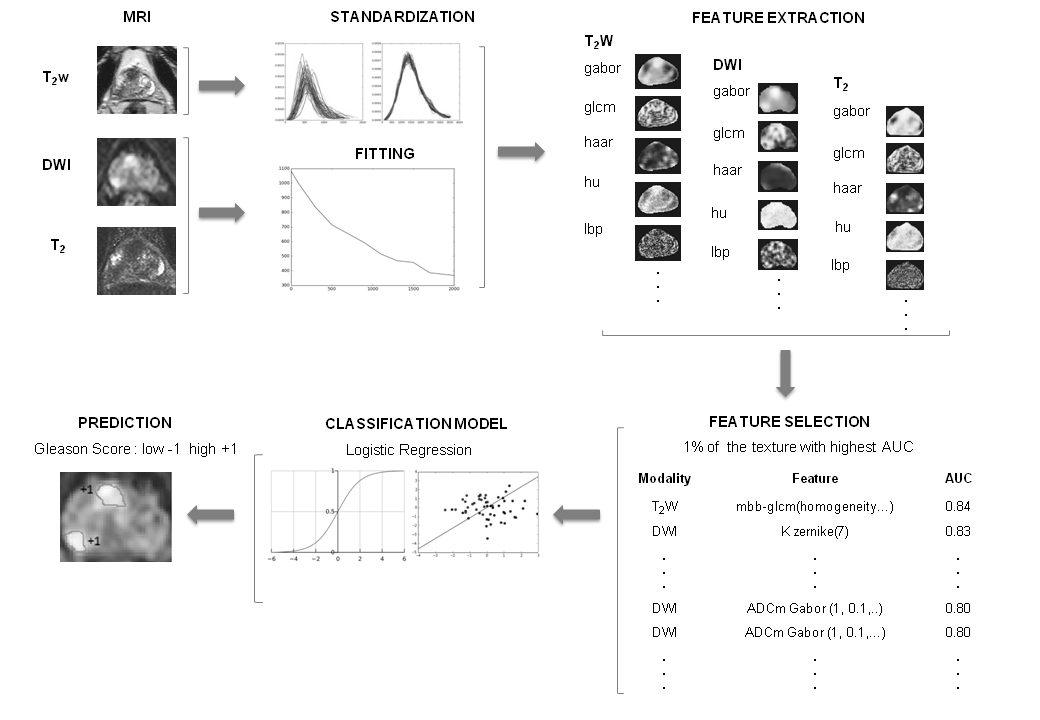
\includegraphics[width=1.0\textwidth]{figures/fig1}

\caption{The post-processing pipeline. The T₂-weighted imaging (T₂w) data set
is standardized while the monoexponential and kurtosis models are applied to
diffusion weighted imaging (DWI) data set. The T₂ relaxation values are obtained
using a two parameter monoexponential function. Subsequently, the features are
calculated using T₂w and parametric maps. The feature selection is performed
by choosing 1\% of the features with highest AUC\@. Then with the selected
features a logistic regression model is fitted and used to predict the lesion's
Gleason score group.}\label{fig:pipeline}

\end{figure}


\begin{figure}[ht]

\centering 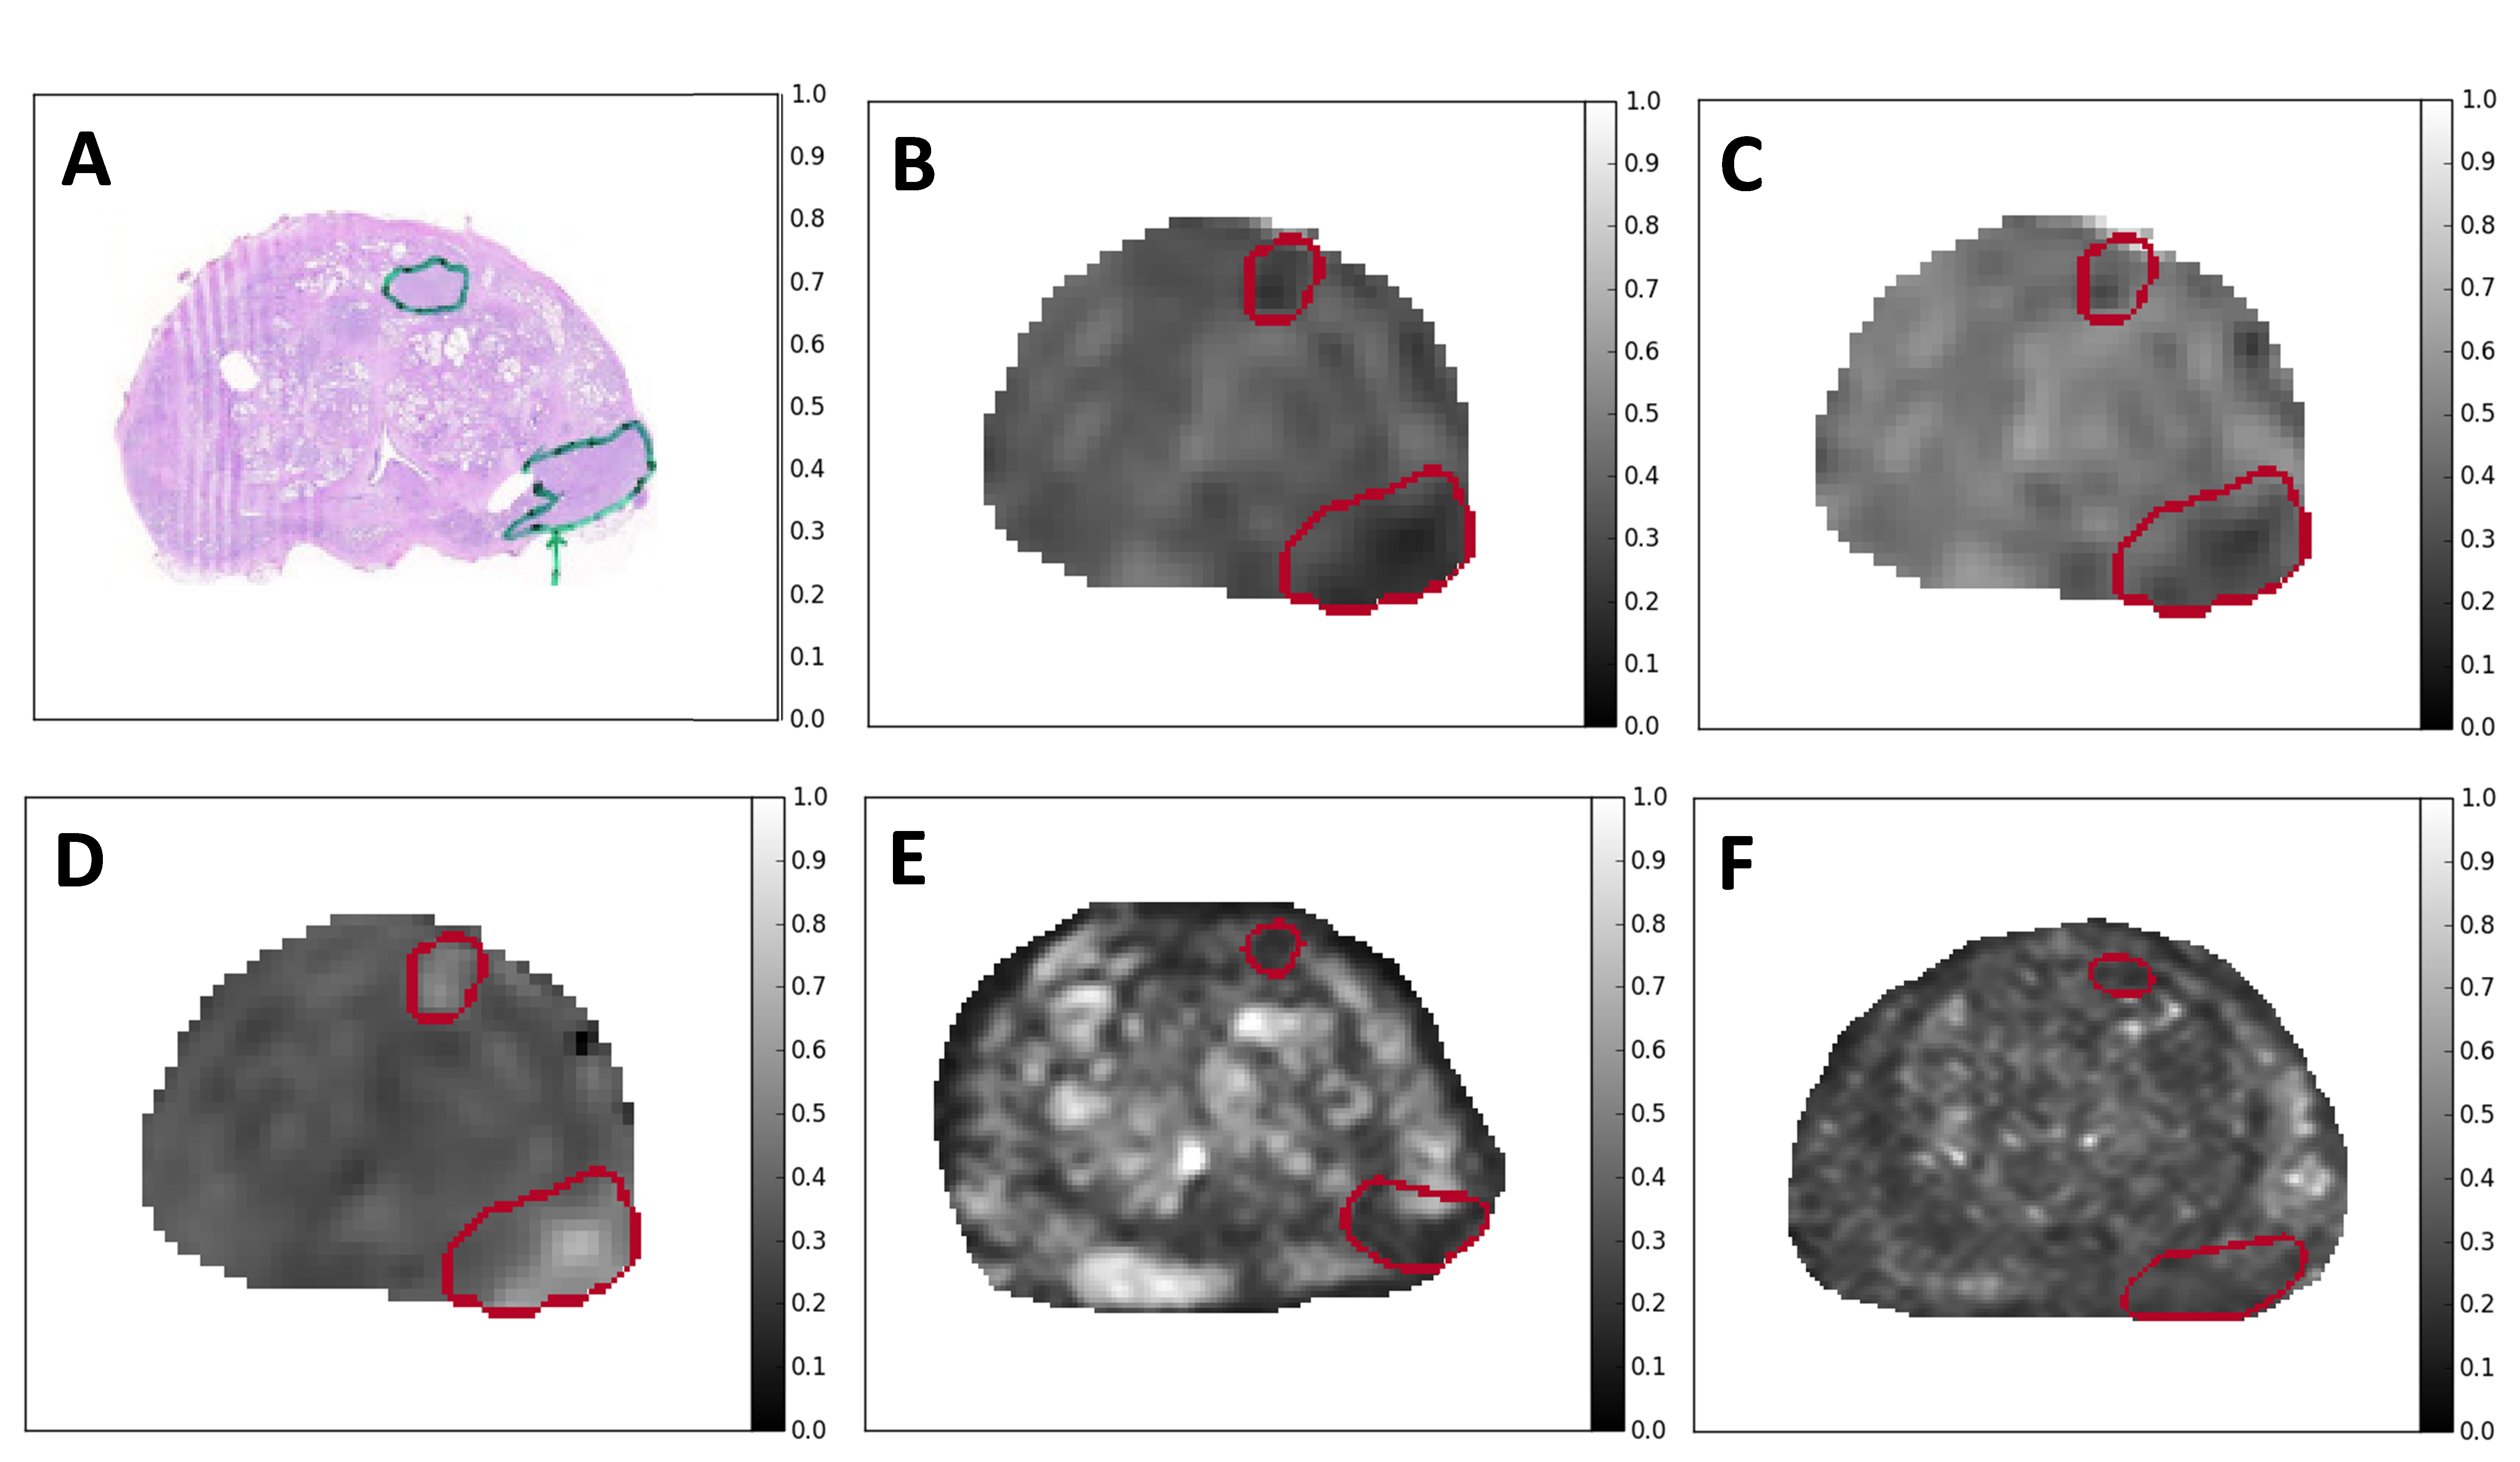
\includegraphics[width=1.0\textwidth]{figures/fig2}

\caption{An example of a whole mount prostate histological section~(A), with
corresponding parametric maps for ADCₘ~(B), ADCₖ~(C), K~(D), T₂w~(E)
and T₂~(F). This is from patient number 43 in Table S1. The two lesions are
outlined; their Gleason scores are 4+3 (lower, in posterolateral region) and 3+4
(upper, in anterior region).}\label{fig:pmap}

\end{figure}


\begin{figure}[ht]

\centering 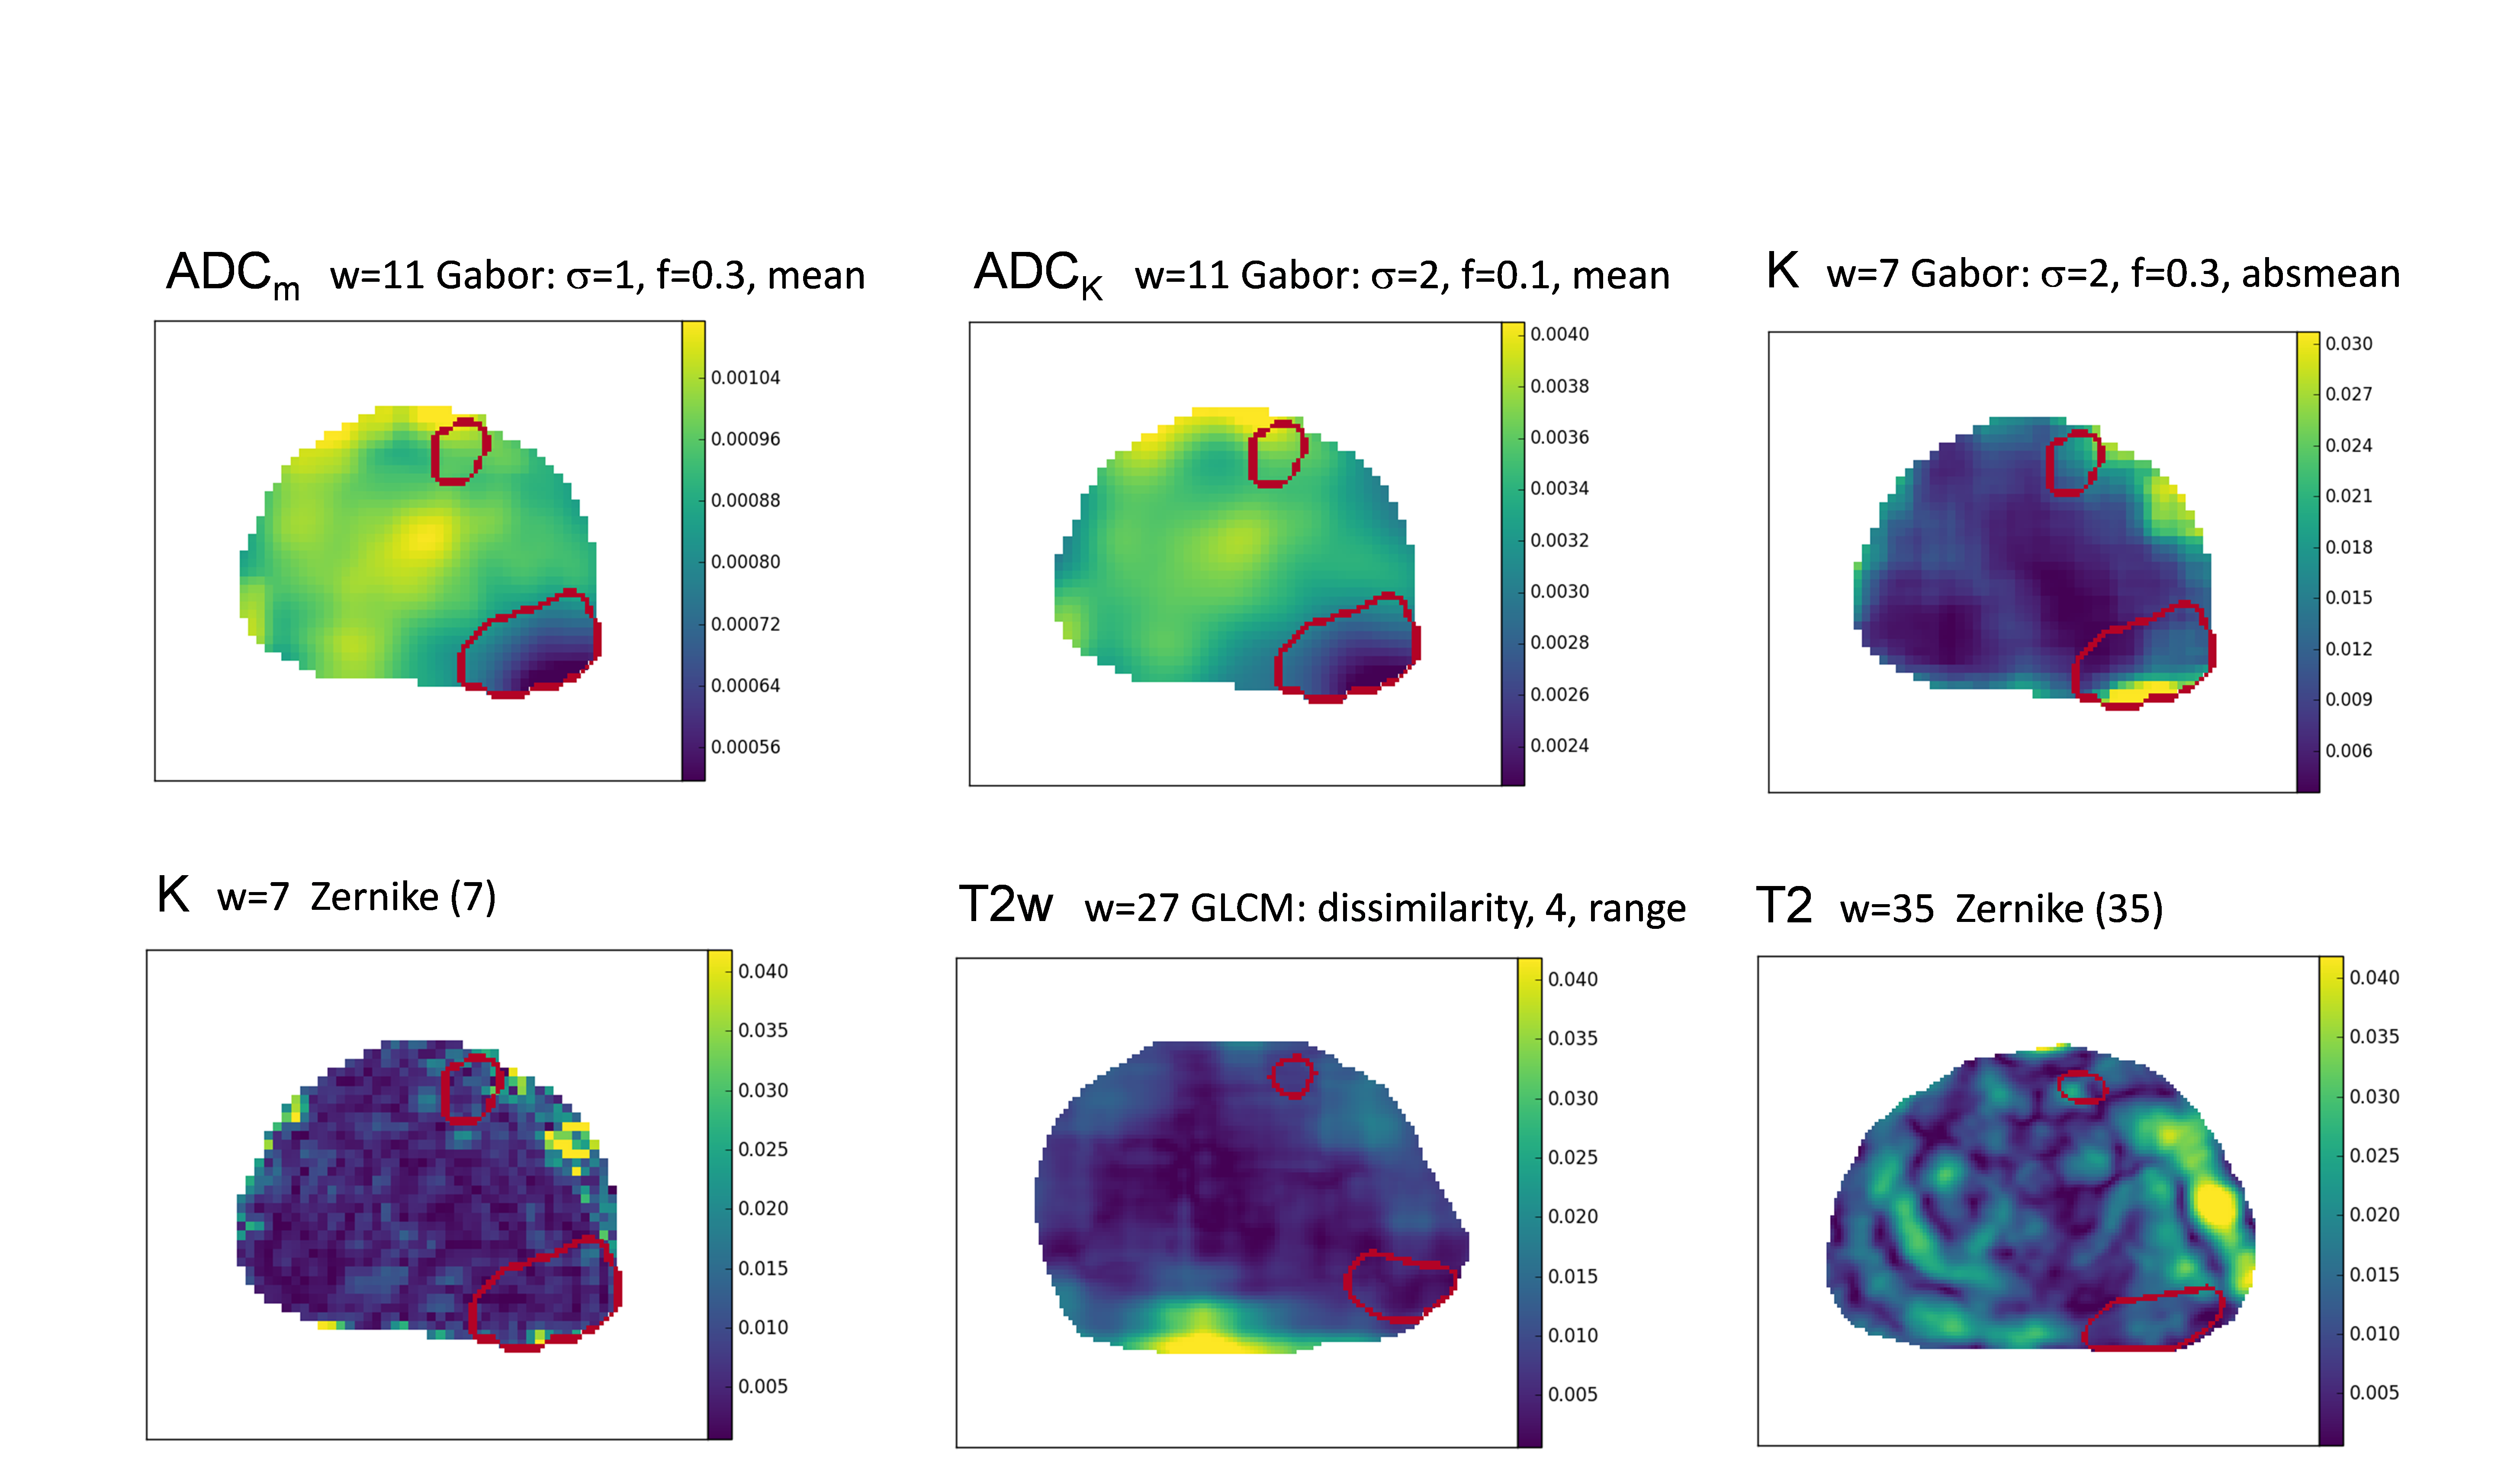
\includegraphics[width=1.0\textwidth]{figures/fig3}

\caption{An example of prostate texture feature maps extracted from DWI
parametric maps (ADCₘ, ADCₖ, K), T₂-weighted imaging (T₂w), and parametric map
of T₂ relaxation values (T₂). Source image type, window size, and texture
descriptor parameters are shown above the images. The two lesions are outlined;
their Gleason scores are 4+3 (lower) and 3+4 (upper).}\label{fig:tmap}

\end{figure}


\begin{figure}[ht]

\centering 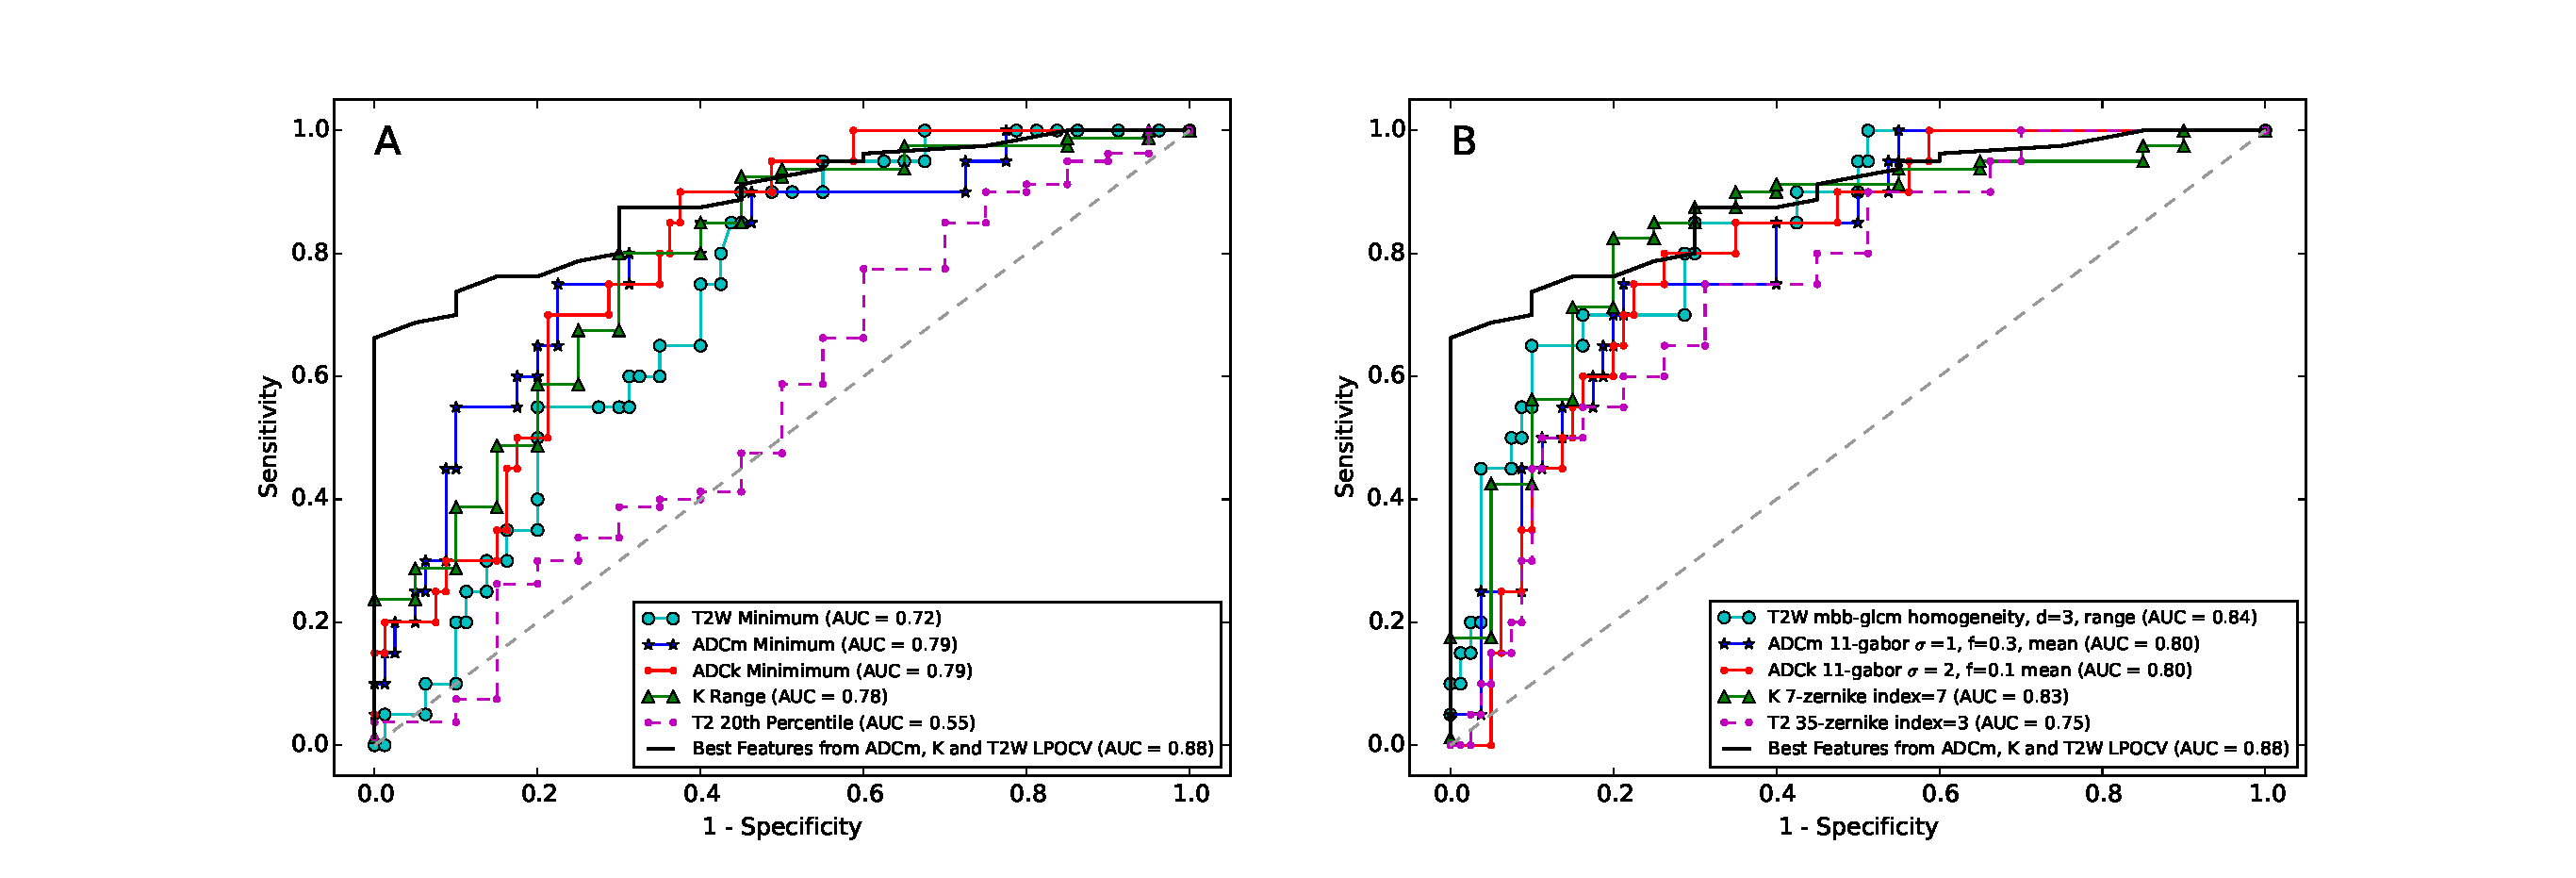
\includegraphics[width=1.0\textwidth]{figures/fig4}

\caption{The ROC curves for the best statistical feature (A) and the best
texture feature (B) within each image type (T₂w, ADCₘ, ADCₖ, K, T₂). The final
model of the best selected features from ADCₘ, K, and T₂w obtained using L1
regularized logistic regression and validated with leave-pair-out
cross-validation (LPOCV) is also included in both A and~B.}\label{fig:roc}

\end{figure}

\newcommand{\fig}[2]{\item Patient #1: #2 map, prostate mask, lesion masks.}
\newcommand{\figADCm}[1]{\fig{#1}{ADCₘ}}
\newcommand{\figTtw}[1]{\fig{#1}{T₂w}}
\newcommand{\figTt}[1]{\fig{#1}{T₂}}

\newcommand{\histology}[2]{\item Patient #1: #2.}
\newcommand{\pink}[1]{\histology{#1}{prostatectomy section}}


\section{Supporting Material captions}

\subsection{Supporting Tables}

\begin{enumerate}
\item Patient characteristics.
\item T₂-weighted imaging: best 5\% features.
\item T₂-weighted imaging: statistical features.
\item Apparent diffusion coefficient of the monoexponential model (ADCₘ): best
  5\% features.
\item Apparent diffusion coefficient of the monoexponential model (ADCₘ):
  statistical features.
\item Apparent diffusion coefficient of the kurtosis model (ADCₖ): best 5\%
  features.
\item Apparent diffusion coefficient of the kurtosis model (ADCₖ): statistical
  features.
\item Kurtosis parameter of the kurtosis model (K): best 5\% features.
\item Kurtosis parameter of the kurtosis model (K): statistical features.
\item T₂ relaxation values (T₂): best 5\% features.
\item T₂ relaxation values (T₂): statistical features.
\end{enumerate}


\subsection{Supporting Figures}

\begin{enumerate}
\figADCm{01} \figADCm{02} \figADCm{03} \figADCm{04} \figADCm{05}
\figADCm{06} \figADCm{07} \figADCm{08} \figADCm{09} \figADCm{10}
\figADCm{11} \figADCm{12} \figADCm{13} \figADCm{14} \figADCm{15}
\figADCm{16} \figADCm{17} \figADCm{18} \figADCm{19} \figADCm{20}
\figADCm{21} \figADCm{22} \figADCm{23} \figADCm{24} \figADCm{25}
\figADCm{26} \figADCm{27} \figADCm{28} \figADCm{29} \figADCm{30}
\figADCm{31} \figADCm{32} \figADCm{33} \figADCm{34} \figADCm{35}
\figADCm{36} \figADCm{37} \figADCm{38} \figADCm{39} \figADCm{40}
\figADCm{41} \figADCm{42} \figADCm{43} \figADCm{44} \figADCm{45}
\figADCm{46} \figADCm{47} \figADCm{48} \figADCm{49} \figADCm{50}
\figADCm{51} \figADCm{52} \figADCm{53} \figADCm{54} \figADCm{55}
\figADCm{56} \figADCm{57} \figADCm{58} \figADCm{59} \figADCm{60}
\figADCm{61} \figADCm{62}
\figTtw{01} \figTtw{02} \figTtw{03} \figTtw{04} \figTtw{05}
\figTtw{06} \figTtw{07} \figTtw{08} \figTtw{09} \figTtw{10}
\figTtw{11} \figTtw{12} \figTtw{13} \figTtw{14} \figTtw{15}
\figTtw{16} \figTtw{17} \figTtw{18} \figTtw{19} \figTtw{20}
\figTtw{21} \figTtw{22} \figTtw{23} \figTtw{24} \figTtw{25}
\figTtw{26} \figTtw{27} \figTtw{28} \figTtw{29} \figTtw{30}
\figTtw{31} \figTtw{32} \figTtw{33} \figTtw{34} \figTtw{35}
\figTtw{36} \figTtw{37} \figTtw{38} \figTtw{39} \figTtw{40}
\figTtw{41} \figTtw{42} \figTtw{43} \figTtw{44} \figTtw{45}
\figTtw{46} \figTtw{47} \figTtw{48} \figTtw{49} \figTtw{50}
\figTtw{51} \figTtw{52} \figTtw{53} \figTtw{54} \figTtw{55}
\figTtw{56} \figTtw{57} \figTtw{58} \figTtw{59} \figTtw{60}
\figTtw{61} \figTtw{62}
\figTt{01} \figTt{02} \figTt{03} \figTt{04} \figTt{05}
\figTt{06} \figTt{07} \figTt{08} \figTt{09} \figTt{10}
\figTt{11} \figTt{12} \figTt{13} \figTt{14} \figTt{15}
\figTt{16} \figTt{17} \figTt{18} \figTt{19} \figTt{20}
\figTt{21} \figTt{22} \figTt{23} \figTt{24} \figTt{25}
\figTt{26} \figTt{27} \figTt{28} \figTt{29} \figTt{30}
\figTt{31} \figTt{32} \figTt{33} \figTt{34} \figTt{35}
\figTt{36} \figTt{37} \figTt{38} \figTt{39} \figTt{40}
\figTt{41} \figTt{42} \figTt{43} \figTt{44} \figTt{45}
\figTt{46} \figTt{47} \figTt{48} \figTt{49} \figTt{50}
\figTt{51} \figTt{52} \figTt{53} \figTt{54} \figTt{55}
\figTt{56} \figTt{57} \figTt{58} \figTt{59} \figTt{60}
\figTt{61} \figTt{62}
\pink{01} \pink{02} \pink{03} \pink{04} \pink{05}
\pink{06} \pink{07} \pink{08} \pink{09} \pink{10}
\pink{11} \pink{12} \pink{13} \pink{14} \pink{15}
\pink{16} \pink{17} \pink{18} \pink{19} \pink{20}
\pink{21} \pink{22} \pink{23} \pink{24} \pink{25}
\pink{26} \pink{27} \pink{28} \pink{29} \pink{30}
\pink{31} \pink{32} \pink{33} \pink{34} \pink{35}
\pink{36} \pink{37} \pink{38} \pink{39} \pink{40}
\pink{41} \pink{42} \pink{43} \pink{44} \pink{45}
\pink{46} \pink{47} \pink{48} \pink{49} \pink{50}
\pink{51} \pink{52} \pink{53} \pink{54} \pink{55}
\pink{56} \pink{57} \pink{58} \pink{59} \pink{60}
\pink{61} \pink{62}
\end{enumerate}


\section*{References}
\bibliography{library}

\end{document}
